\documentclass[11pt,a4paper,titlepage]{article}

\usepackage[letterpaper,top=1in, bottom=1in, left=1.5in, right=1in]{geometry}
\usepackage{url}
\usepackage{setspace}
\usepackage{listings,multicol}
\usepackage{authoraftertitle}
\usepackage{graphicx}
\usepackage{array}
\usepackage[table]{xcolor} 
\usepackage[nottoc,numbib]{tocbibind}
\usepackage{tocloft} 
\setlength{\cftsecnumwidth}{1.2cm}
\setlength{\cftsubsecindent}{1.2cm}
\renewcommand{\refname}{Bibliography}
\renewcommand\thesection{\Roman{section}.}
\renewcommand\thesubsection{\Alph{subsection}.}
\renewcommand\thesubsubsection{\arabic{subsubsection}.}

\doublespacing

\title {Mammo: An Application of Convolutional Neural Networks on Breast Cancer Screening}
\author {Sigfreed John S. Angeles}
\date{June 2018}

% allows for separate page section by changing the behavior of \section
\let\stdsection\section
\renewcommand\section{\newpage\stdsection}
%Acceptance Sheet Template (UP Manila CompSci)
%use %Acceptance Sheet Template (UP Manila CompSci)
%use %Acceptance Sheet Template (UP Manila CompSci)
%use \input{acceptancesheet.tex} in main file
%define title and other parameters using
% \defsptitle
% \defadviserblank
% \defadviser
% \defunitheadblank
% \defunithead
% \defchairblank
% \defchair
% \defdean
% \defdeanblank
% \defpanelone ... \defpanelseven
% in preamble of main file
%use \acceptancesheet to create acceptance sheet at wanted location

%variables
%\usepackage{setspace}
%\usepackage[top=1in, left=1.5in, right=1in, bottom=1in]{geometry}

\newcommand{\defsptitle}[1]{\def \sptitle {#1}}

\newcommand{\defauthor}[1]{\def \authorname {#1 }}

\newcommand{\defadviserblank}[1]{\def \adviserblank {#1}} %Define the size of the blank for the adviser
\newcommand{\defadviser}[1]{\def \adviser {#1}} %Adviser Name

\newcommand{\defunitheadblank}[1]{\def \unitheadblank {#1}} %Define the size of the blank for the unithead
\newcommand{\defunithead}[1]{\def \unithead {#1}} %Unit Head Name

\newcommand{\defchairblank}[1]{\def \chairblank {#1}} %Define the size of the blank for the Dep Chair
\newcommand{\defchair}[1]{\def \chair {#1}} %Unit Head Name

\newcommand{\defdeanblank}[1]{\def \deanblank {#1}} %Define the size of the blank for the dean
\newcommand{\defdean}[1]{\def \dean {#1}} %Dean Name

%Panel Members

\newcommand{\defpanelone}[1]{\def \panelone {#1}}
\newcommand{\defpaneltwo}[1]{\def \paneltwo {#1}}
\newcommand{\defpanelthree}[1]{\def \panelthree {#1}}
\newcommand{\defpanelfour}[1]{\def \panelfour {#1}}
\newcommand{\defpanelfive}[1]{\def \panelfive {#1}}
\newcommand{\defpanelsix}[1]{\def \panelsix {#1}}
\newcommand{\defpanelseven}[1]{\def \panelseven {#1}}

\newcommand{\acceptancesheet}{
\newpage
		\singlespacing
		\begin{center}
			\textbf{ACCEPTANCE SHEET}
		\end{center}
		
		\hspace{4em} The Special Problem entitled ``\MyTitle''$\;$prepared and submitted by \MyAuthor$\;$in partial fulfillment of the requirements for the degree of Bachelor of Science in Computer Science has been examined and is recommended for acceptance.
		\vspace{33pt}	
			\begin{flushright}
						\makebox[0.35\textwidth]{\underline{\hspace{\adviserblank}}}\\	
						\makebox[0.35\textwidth]{\textbf{\adviser}}\\
						\makebox[0.35\textwidth]{Adviser}\\
			\end{flushright}
		\vspace{22pt}
			
			\begin{flushleft}
			\textbf{EXAMINERS:}\\
			\makebox[0.5\textwidth]{}
			\makebox[0.23\textwidth]{\textbf{Approved}}
			\makebox[0.23\textwidth]{\textbf{Disapproved}}\\[22pt]
			
			%Baes
			\makebox[0.5\textwidth][l]{\hspace{0.3cm}1. \panelone}
			\makebox[0.23\textwidth]{\underline{\hspace{2.5cm}}}
			\makebox[0.23\textwidth]{\underline{\hspace{2.5cm}}}\\
			%Carpio
			\makebox[0.5\textwidth][l]{\hspace{0.3cm}2. \paneltwo}
			\makebox[0.23\textwidth]{\underline{\hspace{2.5cm}}}
			\makebox[0.23\textwidth]{\underline{\hspace{2.5cm}}}\\
			%Chua
			\makebox[0.5\textwidth][l]{\hspace{0.3cm}3. \panelthree}
			\makebox[0.23\textwidth]{\underline{\hspace{2.5cm}}}
			\makebox[0.23\textwidth]{\underline{\hspace{2.5cm}}}\\
			%Co
			\makebox[0.5\textwidth][l]{\hspace{0.3cm}4. \panelfour}
			\makebox[0.23\textwidth]{\underline{\hspace{2.5cm}}}
			\makebox[0.23\textwidth]{\underline{\hspace{2.5cm}}}\\
			%Magboo
			\makebox[0.5\textwidth][l]{\hspace{0.3cm}5. \panelfive}
			\makebox[0.23\textwidth]{\underline{\hspace{2.5cm}}}
			\makebox[0.23\textwidth]{\underline{\hspace{2.5cm}}}\\
			%Magboo
			\makebox[0.5\textwidth][l]{\hspace{0.3cm}6. \panelsix}
			\makebox[0.23\textwidth]{\underline{\hspace{2.5cm}}}
			\makebox[0.23\textwidth]{\underline{\hspace{2.5cm}}}\\
			%Terrado
			\makebox[0.5\textwidth][l]{\hspace{0.3cm}7. \panelseven}
			\makebox[0.23\textwidth]{\underline{\hspace{2.5cm}}}
			\makebox[0.23\textwidth]{\underline{\hspace{2.5cm}}}\\[33pt]
					
			\hspace{2em} Accepted and approved as partial fulfillment of the requirements for the degree of Bachelor of Science in Computer Science.\\[44pt]
			
			\makebox[0.48\textwidth]{\underline{\hspace{\unitheadblank}}}
			\makebox[0.48\textwidth]{\underline{\hspace{\chairblank}}}\\
			
			\makebox[0.48\textwidth]{\textbf{\unithead}}
			\makebox[0.48\textwidth]{\textbf{\chair}}\\

			\makebox[0.48\textwidth]{Unit Head}
			\makebox[0.48\textwidth]{Chair}\\
			
			\makebox[0.48\textwidth]{Mathematical and Computing Sciences Unit}
			\makebox[0.48\textwidth]{Department of Physical Sciences}\\
			
			\makebox[0.48\textwidth]{Department of Physical Sciences}
			\makebox[0.48\textwidth]{and Mathematics}
			
			\makebox[0.48\textwidth]{and Mathematics}
			\makebox[0.48\textwidth]{}\\[33pt]
			
			\makebox[\textwidth]{\underline{\hspace{\deanblank}}}
			\makebox[\textwidth]{\textbf{\dean}}
			\makebox[\textwidth]{Dean}
			\makebox[\textwidth]{College of Arts and Sciences}
			
			\end{flushleft}
} in main file
%define title and other parameters using
% \defsptitle
% \defadviserblank
% \defadviser
% \defunitheadblank
% \defunithead
% \defchairblank
% \defchair
% \defdean
% \defdeanblank
% \defpanelone ... \defpanelseven
% in preamble of main file
%use \acceptancesheet to create acceptance sheet at wanted location

%variables
%\usepackage{setspace}
%\usepackage[top=1in, left=1.5in, right=1in, bottom=1in]{geometry}

\newcommand{\defsptitle}[1]{\def \sptitle {#1}}

\newcommand{\defauthor}[1]{\def \authorname {#1 }}

\newcommand{\defadviserblank}[1]{\def \adviserblank {#1}} %Define the size of the blank for the adviser
\newcommand{\defadviser}[1]{\def \adviser {#1}} %Adviser Name

\newcommand{\defunitheadblank}[1]{\def \unitheadblank {#1}} %Define the size of the blank for the unithead
\newcommand{\defunithead}[1]{\def \unithead {#1}} %Unit Head Name

\newcommand{\defchairblank}[1]{\def \chairblank {#1}} %Define the size of the blank for the Dep Chair
\newcommand{\defchair}[1]{\def \chair {#1}} %Unit Head Name

\newcommand{\defdeanblank}[1]{\def \deanblank {#1}} %Define the size of the blank for the dean
\newcommand{\defdean}[1]{\def \dean {#1}} %Dean Name

%Panel Members

\newcommand{\defpanelone}[1]{\def \panelone {#1}}
\newcommand{\defpaneltwo}[1]{\def \paneltwo {#1}}
\newcommand{\defpanelthree}[1]{\def \panelthree {#1}}
\newcommand{\defpanelfour}[1]{\def \panelfour {#1}}
\newcommand{\defpanelfive}[1]{\def \panelfive {#1}}
\newcommand{\defpanelsix}[1]{\def \panelsix {#1}}
\newcommand{\defpanelseven}[1]{\def \panelseven {#1}}

\newcommand{\acceptancesheet}{
\newpage
		\singlespacing
		\begin{center}
			\textbf{ACCEPTANCE SHEET}
		\end{center}
		
		\hspace{4em} The Special Problem entitled ``\MyTitle''$\;$prepared and submitted by \MyAuthor$\;$in partial fulfillment of the requirements for the degree of Bachelor of Science in Computer Science has been examined and is recommended for acceptance.
		\vspace{33pt}	
			\begin{flushright}
						\makebox[0.35\textwidth]{\underline{\hspace{\adviserblank}}}\\	
						\makebox[0.35\textwidth]{\textbf{\adviser}}\\
						\makebox[0.35\textwidth]{Adviser}\\
			\end{flushright}
		\vspace{22pt}
			
			\begin{flushleft}
			\textbf{EXAMINERS:}\\
			\makebox[0.5\textwidth]{}
			\makebox[0.23\textwidth]{\textbf{Approved}}
			\makebox[0.23\textwidth]{\textbf{Disapproved}}\\[22pt]
			
			%Baes
			\makebox[0.5\textwidth][l]{\hspace{0.3cm}1. \panelone}
			\makebox[0.23\textwidth]{\underline{\hspace{2.5cm}}}
			\makebox[0.23\textwidth]{\underline{\hspace{2.5cm}}}\\
			%Carpio
			\makebox[0.5\textwidth][l]{\hspace{0.3cm}2. \paneltwo}
			\makebox[0.23\textwidth]{\underline{\hspace{2.5cm}}}
			\makebox[0.23\textwidth]{\underline{\hspace{2.5cm}}}\\
			%Chua
			\makebox[0.5\textwidth][l]{\hspace{0.3cm}3. \panelthree}
			\makebox[0.23\textwidth]{\underline{\hspace{2.5cm}}}
			\makebox[0.23\textwidth]{\underline{\hspace{2.5cm}}}\\
			%Co
			\makebox[0.5\textwidth][l]{\hspace{0.3cm}4. \panelfour}
			\makebox[0.23\textwidth]{\underline{\hspace{2.5cm}}}
			\makebox[0.23\textwidth]{\underline{\hspace{2.5cm}}}\\
			%Magboo
			\makebox[0.5\textwidth][l]{\hspace{0.3cm}5. \panelfive}
			\makebox[0.23\textwidth]{\underline{\hspace{2.5cm}}}
			\makebox[0.23\textwidth]{\underline{\hspace{2.5cm}}}\\
			%Magboo
			\makebox[0.5\textwidth][l]{\hspace{0.3cm}6. \panelsix}
			\makebox[0.23\textwidth]{\underline{\hspace{2.5cm}}}
			\makebox[0.23\textwidth]{\underline{\hspace{2.5cm}}}\\
			%Terrado
			\makebox[0.5\textwidth][l]{\hspace{0.3cm}7. \panelseven}
			\makebox[0.23\textwidth]{\underline{\hspace{2.5cm}}}
			\makebox[0.23\textwidth]{\underline{\hspace{2.5cm}}}\\[33pt]
					
			\hspace{2em} Accepted and approved as partial fulfillment of the requirements for the degree of Bachelor of Science in Computer Science.\\[44pt]
			
			\makebox[0.48\textwidth]{\underline{\hspace{\unitheadblank}}}
			\makebox[0.48\textwidth]{\underline{\hspace{\chairblank}}}\\
			
			\makebox[0.48\textwidth]{\textbf{\unithead}}
			\makebox[0.48\textwidth]{\textbf{\chair}}\\

			\makebox[0.48\textwidth]{Unit Head}
			\makebox[0.48\textwidth]{Chair}\\
			
			\makebox[0.48\textwidth]{Mathematical and Computing Sciences Unit}
			\makebox[0.48\textwidth]{Department of Physical Sciences}\\
			
			\makebox[0.48\textwidth]{Department of Physical Sciences}
			\makebox[0.48\textwidth]{and Mathematics}
			
			\makebox[0.48\textwidth]{and Mathematics}
			\makebox[0.48\textwidth]{}\\[33pt]
			
			\makebox[\textwidth]{\underline{\hspace{\deanblank}}}
			\makebox[\textwidth]{\textbf{\dean}}
			\makebox[\textwidth]{Dean}
			\makebox[\textwidth]{College of Arts and Sciences}
			
			\end{flushleft}
} in main file
%define title and other parameters using
% \defsptitle
% \defadviserblank
% \defadviser
% \defunitheadblank
% \defunithead
% \defchairblank
% \defchair
% \defdean
% \defdeanblank
% \defpanelone ... \defpanelseven
% in preamble of main file
%use \acceptancesheet to create acceptance sheet at wanted location

%variables
%\usepackage{setspace}
%\usepackage[top=1in, left=1.5in, right=1in, bottom=1in]{geometry}

\newcommand{\defsptitle}[1]{\def \sptitle {#1}}

\newcommand{\defauthor}[1]{\def \authorname {#1 }}

\newcommand{\defadviserblank}[1]{\def \adviserblank {#1}} %Define the size of the blank for the adviser
\newcommand{\defadviser}[1]{\def \adviser {#1}} %Adviser Name

\newcommand{\defunitheadblank}[1]{\def \unitheadblank {#1}} %Define the size of the blank for the unithead
\newcommand{\defunithead}[1]{\def \unithead {#1}} %Unit Head Name

\newcommand{\defchairblank}[1]{\def \chairblank {#1}} %Define the size of the blank for the Dep Chair
\newcommand{\defchair}[1]{\def \chair {#1}} %Unit Head Name

\newcommand{\defdeanblank}[1]{\def \deanblank {#1}} %Define the size of the blank for the dean
\newcommand{\defdean}[1]{\def \dean {#1}} %Dean Name

%Panel Members

\newcommand{\defpanelone}[1]{\def \panelone {#1}}
\newcommand{\defpaneltwo}[1]{\def \paneltwo {#1}}
\newcommand{\defpanelthree}[1]{\def \panelthree {#1}}
\newcommand{\defpanelfour}[1]{\def \panelfour {#1}}
\newcommand{\defpanelfive}[1]{\def \panelfive {#1}}
\newcommand{\defpanelsix}[1]{\def \panelsix {#1}}
\newcommand{\defpanelseven}[1]{\def \panelseven {#1}}

\newcommand{\acceptancesheet}{
\newpage
		\singlespacing
		\begin{center}
			\textbf{ACCEPTANCE SHEET}
		\end{center}
		
		\hspace{4em} The Special Problem entitled ``\MyTitle''$\;$prepared and submitted by \MyAuthor$\;$in partial fulfillment of the requirements for the degree of Bachelor of Science in Computer Science has been examined and is recommended for acceptance.
		\vspace{33pt}	
			\begin{flushright}
						\makebox[0.35\textwidth]{\underline{\hspace{\adviserblank}}}\\	
						\makebox[0.35\textwidth]{\textbf{\adviser}}\\
						\makebox[0.35\textwidth]{Adviser}\\
			\end{flushright}
		\vspace{22pt}
			
			\begin{flushleft}
			\textbf{EXAMINERS:}\\
			\makebox[0.5\textwidth]{}
			\makebox[0.23\textwidth]{\textbf{Approved}}
			\makebox[0.23\textwidth]{\textbf{Disapproved}}\\[22pt]
			
			%Baes
			\makebox[0.5\textwidth][l]{\hspace{0.3cm}1. \panelone}
			\makebox[0.23\textwidth]{\underline{\hspace{2.5cm}}}
			\makebox[0.23\textwidth]{\underline{\hspace{2.5cm}}}\\
			%Carpio
			\makebox[0.5\textwidth][l]{\hspace{0.3cm}2. \paneltwo}
			\makebox[0.23\textwidth]{\underline{\hspace{2.5cm}}}
			\makebox[0.23\textwidth]{\underline{\hspace{2.5cm}}}\\
			%Chua
			\makebox[0.5\textwidth][l]{\hspace{0.3cm}3. \panelthree}
			\makebox[0.23\textwidth]{\underline{\hspace{2.5cm}}}
			\makebox[0.23\textwidth]{\underline{\hspace{2.5cm}}}\\
			%Co
			\makebox[0.5\textwidth][l]{\hspace{0.3cm}4. \panelfour}
			\makebox[0.23\textwidth]{\underline{\hspace{2.5cm}}}
			\makebox[0.23\textwidth]{\underline{\hspace{2.5cm}}}\\
			%Magboo
			\makebox[0.5\textwidth][l]{\hspace{0.3cm}5. \panelfive}
			\makebox[0.23\textwidth]{\underline{\hspace{2.5cm}}}
			\makebox[0.23\textwidth]{\underline{\hspace{2.5cm}}}\\
			%Magboo
			\makebox[0.5\textwidth][l]{\hspace{0.3cm}6. \panelsix}
			\makebox[0.23\textwidth]{\underline{\hspace{2.5cm}}}
			\makebox[0.23\textwidth]{\underline{\hspace{2.5cm}}}\\
			%Terrado
			\makebox[0.5\textwidth][l]{\hspace{0.3cm}7. \panelseven}
			\makebox[0.23\textwidth]{\underline{\hspace{2.5cm}}}
			\makebox[0.23\textwidth]{\underline{\hspace{2.5cm}}}\\[33pt]
					
			\hspace{2em} Accepted and approved as partial fulfillment of the requirements for the degree of Bachelor of Science in Computer Science.\\[44pt]
			
			\makebox[0.48\textwidth]{\underline{\hspace{\unitheadblank}}}
			\makebox[0.48\textwidth]{\underline{\hspace{\chairblank}}}\\
			
			\makebox[0.48\textwidth]{\textbf{\unithead}}
			\makebox[0.48\textwidth]{\textbf{\chair}}\\

			\makebox[0.48\textwidth]{Unit Head}
			\makebox[0.48\textwidth]{Chair}\\
			
			\makebox[0.48\textwidth]{Mathematical and Computing Sciences Unit}
			\makebox[0.48\textwidth]{Department of Physical Sciences}\\
			
			\makebox[0.48\textwidth]{Department of Physical Sciences}
			\makebox[0.48\textwidth]{and Mathematics}
			
			\makebox[0.48\textwidth]{and Mathematics}
			\makebox[0.48\textwidth]{}\\[33pt]
			
			\makebox[\textwidth]{\underline{\hspace{\deanblank}}}
			\makebox[\textwidth]{\textbf{\dean}}
			\makebox[\textwidth]{Dean}
			\makebox[\textwidth]{College of Arts and Sciences}
			
			\end{flushleft}
}

% **********************************************************************************************************
% Update the following to your SP details
\defsptitle{Mammo: An Application of Convolutional Neural Networks on Breast Cancer Screening}
\defauthor{Sigfreed John S. Angeles}
\defadviserblank{6.5cm}
\defadviser{Vincent Peter C. Magboo, M.D., M.Sc.}
\defunitheadblank{6.55cm}
\defunithead{Ma. Sheila A. Magboo, M.Sc.}
\defchairblank{6.5cm}
\defchair{Marcelina B. Lirazan, Ph.D.}
\defdeanblank{6.5cm}
\defdean{Leonardo R. Estacio Jr., Ph.D.}

\defpanelone{Gregorio B. Baes, Ph.D. (\textit{cand.})}
\defpaneltwo{Avegail D. Carpio, M.S.}
\defpanelthree{Richard Bryann L. Chua, Ph.D. (\textit{cand.})}
\defpanelfour{Perlita E. Gasmen, M.S. (\textit{cand.})}
\defpanelfive{Marvin John C. Ignacio, M.S. (\textit{cand.})}
\defpanelsix{Ma. Sheila A. Magboo, M.S.}
\defpanelseven{Geoffrey A. Solano, Ph.D. (\textit{cand.})}
% **********************************************************************************************************

\newcommand{\Keywords}[1]{\par\noindent 
{\small{\em Keywords\/}: #1}}

\usepackage{bm}
\newcommand{\+}{\discretionary{\mbox{${\bm\cdot}\mkern-1mu$}}{}{}}

\lstset{basicstyle=\tiny,columns=flexible,tabsize=1,breaklines=true}

\begin{document}
%\maketitle
\begin{titlepage}

\begin{center}


% Upper part of the page

\textsc{\large University of the Philippines Manila}\\
\textsc{\large College of Arts and Sciences}\\
\textsc{\large Department of Physical Sciences and Mathematics}\\[3.5cm]

% Title
\textsc{\Large \MyTitle}\\[3.5cm]

A special problem in partial fulfillment\\
of the requirements for the degree of\\
\textbf{Bachelor of Science in Computer Science}


\vfill

% Bottom of the page
Submitted by:\\[1.25cm]
\MyAuthor\\
{\MyDate}
\\[1cm]
Permission is given for the following people to have access to this SP:
\\[0.5cm]
\begin{tabular}{|c|c|}
	\hline
	Available to the general public & Yes \\
	\hline
	Available only after consultation with author/SP adviser & No \\
	\hline
	Available only to those bound by confidentiality agreement & No \\
	\hline
\end{tabular}

\end{center}

\end{titlepage}
\pagenumbering{roman}

\addcontentsline{toc}{section}{Acceptance Sheet}
\acceptancesheet

\doublespacing

\begin{abstract}
\addcontentsline{toc}{section}{Abstract}
\thispagestyle{plain}
\setcounter{page}{2}
	\qquad In screening mammography for breast cancer, radiologists often identify the region of interest (ROI) in a mammogram, and analyze it whether it's benign or malignant, and whether it's a mass or calcification abnormality, for the course of treatment is dependent on the result of the exam. However, there are cases where the ROI is extremely difficult to classify, and radiologists sometimes have conflicting readings. Consequently, Mammo, an application that utilized Convolutional Neural Networks (CNN), was created in this study providing radiologists and medical field students/trainees a tool for classifying their mammograms as well as an exam for the students/trainees. The CNN architecture used was ResNet-50, a CNN where layers can be stacked without the typical vanishing or exploding gradients problem that plague CNNs when more layers are stacked. Using CBIS-DDSM (Curated Breast Imaging Subset of the Digital Database for Screening Mammography), initially, the network achieved an accuracy rate of 33\%. This is caused by lack of data augmenting technique performed on the dataset as well as an imabalance of instances per category. After balancing the instances, CNN ResNet-50 achieved an overall accuracy rate of 43\%.
\Keywords{breast cancer, mammography, convolutional neural network, resnet-50, mass, calcification, benign, malignant, data augmentation}
\end{abstract}

\pagenumbering{roman}
\setcounter{page}{3}
\setcounter{tocdepth}{3}
\newpage
\tableofcontents
\newpage
\listoffigures

\doublespacing

\section{Introduction}
\pagenumbering{arabic}
\setcounter{page}{1}
\subsection{Background of the Study}
\qquad Breast cancer is an uncontrolled growth of breast cells. These cells are also known as malignant tumors. On the other hand, benign tumors are not considered cancerous because their cells are close to normal in appearance; they grow slowly; and they do not invade nearby tissues or spread to other parts of the body. On the other hand, malignant tumors are cancerous due to the cells spreading to distant areas of the body. \cite{breastCancer}. \\

	To date, the precise causes of breast cancer are unknown. But there are known main risk factors attributed to breast cancer. Among the most significant factors are advancing age and a family background of breast cancer. Other factors include hormonal, lifestyle, and environmental factors. Still, most women considered at high risk for acquiring best cancer do not get it, while many with no known risk factors do develop breast cancer \cite{cause}. \\

	Early symptoms and signs of breat cancer are usually unrecognizable. There are also some reports of larger breast cancer cases not producing symptoms and signs. When sypmtoms do occur, the most common symptom is a lump or mass in the breast or underarm area. Other symptoms include nipple discharge, nipple redness, newly inverted nipple, changes in the breast skin texture such as puckering or dimpling, and swelling of part of the breast \cite{symptoms}. \\

	As for the screening and diagnosis of breast cancer, mammography is the way to go. Mammography is a specialized medical imaging that uses a low-dose x-ray system to see inside the breasts. Screening mammography is imperative in early detection of breast cancers because it can show changes in the breast up to two years before a patient or physician can feel them. Furthermore, early detection of breast cancer is crucial because it is at that phase when they are most curable \cite{screeningMammography}. Other common methods of breast cancer screening include a clinical breast exam, breast magnetic resonance imaging (MRI), and breast ultrasound. \\

	In this study, there are two common types of abnormalities that may be observed in screening mammography namely calcification cases and mass cases. Breast calcifications are small spots of calcium salts \cite{calcification} whereas masses are three-dimensional lesions. Given this, four classifications can be made from a region of interest (ROI) in any mammogram specifically benign mass, malignant mass, benign calcification, and malignant calcification. In mammogram analysis, round, oval, or lobulated masses with defined margins or borders are benign tumors. Moreover, larger calcifications with regular or oval shapes are benign, while smaller, irregular calcifications are potentially malignant. \\

	Recently, there have been advances in breast cancer treatment technology providing more options for those afflicted. These options include surgery (mastectomy and lumpectomy), radiation therapy, hormonal (anti-estrogen) therapy, chemotherapy, and targeted therapy \cite{treatmentOptions}. However, the kind of treatment to be recommended depends on the type of breast cancer, the size of the tumor, and the stage of the breast cancer \cite{treatmentHow}. \\
	
	In the United States alone, the estimated number of new cases for 2018 is 266,120 for both men and women with women being the majority (268,670). It is also estimated that 40,920 deaths will arise from this \cite{statistics}. Moreover, the Philippines was declared the country with the most number of cases of breast cancer out of 197 countries in 2016 according to data released by Philippine Obstetrical and Gynecological Society \cite{prevalencePH}. Moreover, the Philippines has the highest incidence of breast cancer in Asia with one in every 13 Filipino women at risk of being afflicted with the disease \cite{incidencePH}. \\

	The high incidence of breast cancer brings not only financial troubles to the affected families but economic repercussions to the country as well. In 2015, a news article reports about an action study, Asia Costs in Oncology, conducted across eight countries in Southeast Asia: Cambodia, Indonesia, Laos, Malaysia, Mayanmar, Thailand, Vietnam, and the Philippines. The study aimed at assessing the impact of cancer on household economic wellbeing, patient survival, and quality of life. The results of the study showed that of the 9,513 patients followed up at 12 months after cancer diagnosis in SEA, over 75 percent of patients had the worst outcomes specifically 29\% died of cancer while 48\% experienced financial catastrophe \cite{cancerBurden}. \\

	With the advent of machine learning, there have been several applications of machine learning algorithms specifically artificial neural networks (ANN) for data problems such as image processing, character recognition, and forecasting (i.e. predicting stock prices). Recently, the research on ANN has lead to the development of a new form of machine learning specifically deep learning through convolutional neural networks (CNN) \cite{applicationML}. CNN has been developed by Szegedy et al., and is the most popular neural network architecture for deep learning for images. One advantage of CNNs compared to ANNs is the robustness of CNNs in image detection especially when dealing with distortions such as changes in shape due to camera lens, different lighting conditions, different poses, presence of partial occlusions, horizontal and vertical shifts, etc. This entails better generalization of a model. Another main advantage is that CNNs have significantly fewer parameters than ANNs, therefore memory requirements are drastically reduced. And, since the number of parameters would be much lower, training time is proportionately reduced \cite{ANNvsCNN}. \\

	Some recent applications of CNN for medical imaging include the diagnosis of Malaria through blood smear images \cite{malariablood}, Thorax disease through chest x-ray images \cite{thorax}, and Helicobacter pylori gastritis through endoscopic images \cite{helicobacter}. Moreover, there are also several CNN applications for medical imaging for breast cancer screening. Given this, an expert system with a CNN application for mammogram screening should be feasible. \\

	In 2015, a Residual Neural Network (RNN), a type of CNN, called ResNet-152 developed by Microsoft won the ImageNet Large Scale Visual Recognition Competition (ILSVRC), where it topped with a top-5 error rate of 3.57\% beating human-level performance on the ImageNet data set. Moreover, ResNet-152 outperformed other popular CNN architectures such as GoogleNet, VGG, and AlexNet by incorporating the residual learning framework. Residual learning allows deeper CNNs to be trained safely without the degradation problem that occurs with the addition of more layers. With deeper CNNs, more complex tasks can be solved, and classification/recognition accuracy also increases \cite{Resnet}. \\

\subsection{Statement of the Problem}
	As stated, mammography is the recommended screening technique. Consequently, the mammogram is analyzed by the radiologist in order to check for lesions and to give a proper reading. However, there are cases where, even with the most experienced of radiologists, it is extremely difficult to identify and distinguish malignant tumors from benign ones. And it is also tedious for a radiologist to analyze a large batch of mammograms if such an event arises.
	Also, more often than not, students or trainees in medical fields would have a difficult time learning concepts and mechanics regarding mammogram screening, since there is a lack of online learning materials for screening mammography especially in the analysis and interpretation of mammograms.

\subsection{Objectives of the Study}
\subsubsection{Training Module}
\qquad This study aims to build an expert system called Mammo through the use of a pretrained CNN and fine-tuning its parameters. The CNN model is slightly patterned off of Shen's pretrained ResNet-50, a RNN with 50 layers, patch classification model \cite{CNNmodel}, since the author trained on the same data set used in this study, CBIS-DDSM (Curated Breast Imaging Subset of the Digital Database for Screening Mammography), and achieved a high accuracy of 0.89. However, the author's model trained on the whole image dataset whereas the model in this study was off of the cropped ROI image version of the dataset. The model was trained given the following details:
	
\begin{enumerate}
	\item Train the network through the gradient descent by back propagation algorithm.
	\item Train the network with the following parameters:
	\begin{enumerate}
		\item Set the learning rate according to 0.001.
		\item Set the total number of epochs to 40.
	\end{enumerate}
	\item Convert the mammograms from DICOM into PNG format in order for the mammogram images to be utilized by pyhton libraries.
	\item Relabeled the images in an iterative manner starting from 0 e.g. 0.png, 1.png, 2.png, etc.
	\item Train the network to classify a ROI into four categories: benign mass, malignant mass, benign calcification, and malignant calcification.
\end{enumerate}

\subsubsection{User Objectives}
	Mammo assists radiologists on the screening of mammograms specifically by providing a support tool to augment radiologist's interpretation particularly in difficult cases. Moreover, this study aims to provide a means for medical students to verify the diagnoses they've made especially when they're undertaking a course in screening mammography:

\begin{enumerate}
	\item Allows the radiologist to
	\begin{enumerate}
		\item Upload and input mammogram/batch of mammograms
		\item View the mammogram/batch of mammograms
		\item Output the classification whether there exists some benign mass, malignant mass, benign calcification, or malignant calcification
		\item Download and save the classification/s made into a PDF file
	\end{enumerate}
	\item Allows students or trainees in medical fields to
	\begin{enumerate}
		\item Upload and input a mammogram/batch of mammograms
		\item View the mammogram/batch of mammograms
		\item Output the classification whether there exists some benign mass, malignant mass, benign calcification, or malignant calcification
		\item Download and save the classification/s made into a PDF file
		\item Test their knowledge of mammograms through a multiple choice quiz
	\end{enumerate}
\end{enumerate}

\subsection{Significance of the Project}
\qquad The expert system assists radiologists by providing a second, unbiased opinion regarding the diagnosis which would improve radiologist's diagnostic confidence. The system may also act as an arbiter for conflicting readings.

	The system can be used as a learning tool for medical students or trainees by providing them an avenue to verify their practice mammogram readings.

\subsection{Scope and Limitations}
\begin{enumerate}
	\item The system is implemented as a web application but would not be publicly distributed.
	\item Only mammograms in PNG, JPG, and JPEG format and have a size of at least 1152x896 are accepted as input.
	\item The network is only trained under CBIS-DDSM.
	\item The network can only make 4 conclusions with regards to the diagnosis of the mammogram/s namely benign mass, malignant mass, benign calcification, and  malignant calcification.
	\item The exam given to the medical field student is only multiple choice, and its question pool is limited.
	\item The system requires the user to specify a ROI from the mammogram for analysis instead of having the whole image analyzed.
\end{enumerate}

\subsection{Assumptions}
\begin{enumerate}
	\item The mammograms that the user would input is assumed to be anonimized or permitted by the patient.
	\item The mammogram can be of the left or right breasts and can be craniocaudal (CC) or mediolateral oblique (MLO).
	\item The system does not cover other means of breast cancer medical imaging such as Magnetic Resonance Imaging (MRI) scans.
	\item The user is assumed to have a built-in NVIDIA graphical processing unit (GPU) in his/her machine.
\end{enumerate}
\section{Review of Related Literature}

\qquad In recent years, there have been an influx of deep learning applications from various researchers for medical imaging tasks. To name a few, Penas et. al \cite{malariablood} implemented a CNN to recognize Malaria parasites on microscopic images of thin blood smears; Shichijo et. al \cite{helicobacter} explored the role of artificial intelligence in the diagnosis of Helicobacter pylori gastritis based on endoscopic images; and Chen et. al \cite{thorax} constructed a deep CNN based method for thorax disease diagnosis through chest x-ray images. \\

	Quinn et. al \cite{quinn} also evaluated the performance of deep CNN on three different microscopic tasks: diagnosis of malaria in thick blood smears, tuberculosis in sputum samples, and intestinal parasite egg in stool samples. The authors also explored methods to maximize the performance of the deep CNN they've constructed. In their methodology, the images were downsampled and then split up into overlapping patches, with the downsampling factor and patch size determined by the type of pathogen to be recognised in each case. This is because each image for each case have several objects (plasmodium for Malaria, Tuberculosis bacilli, and eggs of hookworm) of interest. Through this, the authors have obtained a significantly larger data set. Although the potential number of negative patches (i.e. with absence of any of these pathogens, though possible with other types of objects such as staining artifacts, blood cell or impurities) is disproportionately large compared to the number of positive patches since most of each image do not contain pathogen objects, two measures were done by the authors to make the training and testing sets more balanced. First, negative patches were randomly discarded so that there was at most 100 times the number of positive patches. Second, new positive patches were created by applying data augmenting techniques such as rotating, flipping and a combination of both, yielding 7 extra positive patches for each original one. Their method of generating more instances for the data set is especially useful for when the number of images procured is small. For the results of all cases, accuracy is very high with the AOC scores being greater than 0.99. \\

	Cancer imaging is no exception to deep learning applications. In fact, there have been several studies about deep learning applications for lung cancer, skin cancer, colorectal cancer, bladder cancer, prostate cancer, and breast cancer for the past couple of years. Pearce \cite{pearce} investigated the application of deep learning networks to tumour classification specifically to correctly classify the location of mitoses in slide images. The author found that simple networks can deliver reasonable performance comparable with mid-range performers on the same data set. The simple network constructed in the study is a three-layer convolutional neural network with a binary classifier in the final layer trained on biopsy slide images. The author also explored ways in which model saturation can be resolved. The study suggests that model saturation can be resolved by a combination of limiting the number of parameters in the model, ensuring that training data is balanced between positive and negative instances, low learning rates, and iteratively biasing the input data towards examples that thte model has incorrectly classified after previous training epochs (supervised learning). The resulting model performed reasonably well scoring a 72\% accuracy. \\

	Computer imaging methods in the past fail to consider the difference between natural images and medical images for training CNNs. Moreover, when examining medical images, a set of views must be fused in order to perform a proper reading. Geras et. al \cite{geras} proposed to use a multi-view deep CNN that handles a set of high-resolution medical images specifically a large-scale mammography-based breast cancer screening data set consisting of 886,000 images. The authors built a CNN that classifies an input image as BI-RADS 0 ("incomplete"), BI-RADS 1 ("normal"), or BI-RADS 2 ("benign finding"). The novelty of the authors' method here is that instead of heavily downscaling an original high-resolution image, they kept the input at 2600 x 2000 pixels. Heavily downscaling an image is a common method in object recognition and detection in order to improve the computational efficiency, both in terms of computation and memory, and also because no further improvement has been attributed with higher-resolution images. However, the authors argued that this kind of method works well with natural images where the objects of interest are usually presented in larger portions than other objects, and what matters most are their macro-structures such as shapes, colors, etc. On the other hand, medical images, where there are fine details to consider, do no share these properties with natural images, so the downscaling of medical images are not desirable. The authors used aggresive convolution layers and pooling layers specifically convolution layers with strides larger than one in the first two convolutional layers and the first pooling layer with a larger stride than the other pooling layers. An experiment was conducted where the accuracies where evaluated with different decreases in resolution of the image. The results are that when the images where downscaled by x 1/8, the peak accuracy was 74.3\%. On the other hand, when the images are not downscaled, the peak accuracy was 78.7\%. \\

	In training and fine tuning CNNs, a large amount of labeled data is always required. However, for most medical image projects, acquiring such a database is very difficult. Sun et. al \cite{sun} developed a graph-based semi-supervised learning (SSL) scheme using deep CNN for breast cancer diagnosis. SSL is a technique in machine learning wherein labeled data and unlabeled data are employed in the training of the model. Here, the authors' proposed scheme only requires a small portion of labeled data (100 instances). This is potentially useful and powerful since the process of diagnosing and labeling hundreds or even thousands of data is costly. Consequently, their CNN model achieved an accuracy of 0.8243 and an area under the ROC curve of 0.8818. \\

	According to Chougrad et. al \cite{chougrad}, radiologists often find it difficult to classify mammography mass lesions. So, the authors constructed a Computer Assisted Diagnosis (CAD) system based on a deep CNN model that classifies breast mass lesions. The authors proposed the use of transfer learning with exponentially decaying learning rate per layer. The use of transfer learning was justified by the small size of the data set only comprising of 600 images, 300 images showing benign lesions and 300 showing malignant lesions. Then, when fine-tuning the CNN, the weights of the last convolutional layers need to be tweaked as much as possible, while the first ones remain nearly untouched. They propose to do this by the aforementioned per-layer exponentially decaying learning rate. The rationale for this was that the first layers of CNN learn generic features, while the last layers tend to be more specific to the data hence by fine-tuning the last convolutional layers, the model learns more data-specific features. With the setup they've proposed, their model achieved an accuracy of 98.23\% on an independent, test database. \\

	Araújo et. al \cite{araujo} constructed a CNN for a different task specifically the classification of hematoxylin and eosin stained breast biopsy images into four classes namely normal tissue, benign lesion, in situ carcinoma and invasive carcinoma, and in two classes, carcinoma and non-carcinoma. The architecture of the CNN was custom-tailored to retrieve information at nuclei level and overall tissue organization. This is performed by first processing several patches obtained from an input image with a patch-wise classifier, and then combining the classification results of all the image patches to obtain the final image-wise classification. In addition, the author evaluated the performance of two network architecture, a CNN and a CNN with the feed-forward neural network swapped with a Support Vector Machine (SVM) classifier. Accuracies of 77.8\% for four class and 83.3\% for carcinoma/non-carcinoma are achieved. \\

	Similarly, Rakhlin et. al \cite{rakhlin} had similar objectives to that of Araújo et. al which was to develop a deep CNN for the classification of hematoxylin and eosin stained breast biopsy images into four classes (normal tissue, benign lesion, in situ carcinoma and invasive carcinoma) and in two classes (carcinoma and non-carcinoma). They both had the same data set, 400 images of 4 classes. To remedy the problem of overfitting due to a small data set, the authors employed an approach known as deep convolutional feature representation by which deep CNNs, trained on large and general datasets like ImageNet, are used for unsupervised feature representation extraction. They also used Light GBM, a fast, distributed, high performance implementation of gradient boosted trees, for supervised classification. The results of their model outperformed that of \cite{araujo} having an accuracy of 87.2\% for the 4-class classification task and 93.8\% accuracy for the 2-class classification. \\

	In 2015, He et. al \cite{Resnet} proposed a residual learning framework to achieve deeper CNNs without dealing with vanishing and exploding gradients when training very deep CNNs. They constructed a CNN with shortcut connections that skip one or more stacked layers through use of identity mapping where the outputs of shortcut connections are added to the outputs of the stacked layers. The resulting network is referred to as a residual neural network (RNN). The author's constructed model, a 152-layer RNN, surpassed human-level performance on the ImageNet classification data set with an accuracy of 0.89. \\

	Unfortunately, these studies do not discuss the implementation of their model into a widely-distributed system. However, Weng \cite{weng} was tasked to develop a CNN by iSono Health, a startup company, who developed the iSono app, an affordable, automated ultrasound imaging platform to assist women with monthly self-monitoring of breast cancer detection. The application comes with a device that allows user to self-scan through ultrasound. The resulting images are sent to the user's physician who sends back a diagnosis regarding the images. A well-developed CNN could potentially remove the need for a physician, for the physician is not always readily-available. The objective of the CNN was to differentiate benign and malignant breast lesions. Furthermore, the author compared the performance of a CNN with respect to a fully-connected neural network (FCNN). The CNN model constructed achieved an accuracy of 73\% while the FCNN only achieved 66\%. In the author's paper, there was no discussion regarding the specifics of incorporating the constructed model into the iSono app.  Moreover, the CNN model achieved a relatively low accuracy compared to other models mentioned as the model was built from scratch, and the design was inspired by AlexNet. \\

	Large-scale medical image databases with fully-annotated ROIs are scarce. There are only a handful of such databases that are publicly available such as CBIS-DDSM. It would also be unrealistic to require all existing databases to be fully annotated with ROIs. In \cite{CNNmodel}, Shen developed an end-to-end training algorithm for whole-image breast cancer diagnosis based on mammograms. The authors achieved a trainable whole image classifier model from patch-wise classifier model greatly reducing reliance on data sets with lesion annotations as there are only a few databases that exist with such ROI annotations. This is done by training a patch-wise classifier model first then adding a new convolutional layer on top of the patch-wise classifier. The best constructed whole image classifier model achieved an AUC score of 0.88 on DDSM (Digital Database for Screening Mammography). And, the model was trained as well on INbreast, a database with whole image annotations, which achieved an AUC score of 0.96.
\section{Theoretical Framework}
\subsection{Breast Cancer}
\qquad Breast Cancer is a malignant tumor, a collection of cancer cells, arising from the cells of the breast. Breast cancer typically originates in the cells of the lobules, milk-producing glands, or the ducts, the passages that drain milk from the lobules to the nipple \cite{breastCancer}. \\

	There are several types of breast cancer, but the type of breast cancer is classified by the specific cells in the breast that are afflicted by the disease. The most common types are ductal carcinoma in situ, invasive ductal carcinoma, and invasive lobular carcinoma.The terms "in situ" and "invasive" refer to the extent of the spread of the cancer. "In situ," also called as "non-invasive," means that the cancer has not spread, while "invasive," also called as "infiltrating," means that the cancer has spread to the surrounding breast tissue \cite{breastCancerTypes}.

\begin{enumerate}
	\item \textit{Ductal carcinoma in situ} \\
	Ductal carcinoma in situ (DCIS) is the most common type of non-invasive breast cancer \cite{breastCancerOrgDCIS}. DCIS is described by cancer cells that line the milk ducts of the breast. Since it is non-invasive, it is contained only in the milk ducts, but immediate treatment is still necessary, for it may eventually become invasive \cite{ACSDCIS}.

	\item \textit{Invasive ductal carcinoma} \\
	Invasive ductal carcinoma (IDC) is the most common type of breast cancer accounting for about 80\% of all breast cancers. IDC means that the cancer has spread to the surrounding breast tissue originating from the milk ducts. Over time, the cancer may spread to the lymph nodes and other parts of the body \cite{breastCancerOrgIDC}.

	\item \textit{Invasive lobular carcinoma} \\
	Invasive lobular carcinoma (ILC) is the second most common type of breast cancer after IDC. ILC is characterized by cancer that originated from the lobules. Like IDC, the cancer cells have the potential to spread to the lymph nodes and other areas of the body \cite{breastCancerOrgILC}.
	
\end{enumerate}

	As mentioned, the most common symptom of breast cancer is a new lump or mass. A painless, hard mass with irregular edges is evidently cancer, but, in other breast cancer cases, the mass can be tender, soft, rounded, and painful. Other possible symptoms include:

\begin{itemize}
	\item swelling of all or part of a breast even if no distinct lump is felt
	\item skin irritation or dimpling
	\item breast or nipple pain
	\item nipple retraction
	\item redness, scaliness, or thickening of the nipple or breast skin
	\item nipple discharge
\end{itemize}

	In invasive breast cancer, there are cases where, after spreading to the lymph nodes under the arm or around the collar bone, swelling may occur there, even before the original tumor in the breast becomes large enough to be felt \cite{ACSSymptoms}. \\

	The survival rates for breast cancer depends solely on the stage or the extent of the cancer. Generally, the survival rates are higher for women with earlier stage cancers. According to the National Cancer Institute's SEER database from people diagnosed with breast cancer from 2007 to 2013, the 5-year relative survival rate for women with stage 0 or stage I breast cancer is close to 100\%; the 5-year relative survival rate for women with stage II breast cancer is approximately 93\%; the 5-year survival rate for stage III breast cancers is about 72\%; Lastly, the 5-year relative survival rate for women with stage IV breast cancers is about 22\%. Fortunately, there are many widely available treatment options even for this stage of cancer \cite{cancerPrognosis}. \\

	Treatment depends on the biology and behavior of breast cancer. Treatment options and recommendations are very personalized and depend on several factors \cite{cancerTreatmentSpecific}:

\begin{itemize}
	\item the stage of the tumor
	\item the patient's age, general health, menopausal status, and preferences
	\item the presence of known mutations in inherited breast cancer genes
\end{itemize}

	Cancer care teams comprising of several health care professionals such as surgeons, radiologists, oncologists, physycian assistants, oncology nurses, social workers, pharmacists, counselors, nutritionists, and others work together to create a patient's overall treatment plan which is a summary of planned cancer treatment. Some of the most common treatment options include \cite{cancerTreatmentSpecific}:

\begin{enumerate}
	\item Surgery \\
	Surgery is the removal of the tumor and some surrounding healthy tissue for good measure. There are two type of surgery namely lumpectomy and mastectomy. Lumpectomy is the removal of the tumor and a small, cancer-free area of healthy tissue around the tumor. Often, there could be several follow-up treatments after surgery such as radiation therapy. On the other hand, mastectomy is the surgical removal of the entire breast.

	\item Radiation therapy \\
	Radiation therapy is the use of high-energy x-rays of other particles to destroy cancer cells. Some types include external-beam radiation therapy, intra-operative radiation therapy, and brachytherapy. External-beam radiation therapy is radiation given to the affected area from a machine outside the body. Intra-operative radiation therapy is given using a probe in the operating room. Lastly, brachytherapy is done by placing radioactive sources into the tumor. \\

	Radiation therapy is usually given over a set period of time indicated by the regimen given by the radiation oncologist. However, this kind of treatment may cause side effects such as fatigue, swelling of the breast, redness and/or skin discoloration, and pain/burning in the skin where the radiation was directed.

	\item Chemotherapy \\
	Chemotherapy is the use of drugs to destroy cancer cells usually by inhibiting the cancer cells' ability to grow and spread. The common ways by which chemotherapy drugs are applied include an intravenous tube placed into a vein using a needle, an injection under the skin or into a muscle, or a pill or capsule that is swallowed. Chemotherapy may also be given before surgery to shrink larger tumors to make surgery easier, and after surgery to minimize the risk of recurrence. Common drugs prescribed include capecitabine, carboplatin, cisplatin, cyclophosphamide, docetaxel, doxorubicin, pegylated liposomal doxorubicin, epirubicin, fluorouracil, gemcitabine, methotrexate, paclitaxel, protein-bound paclitaxel, vinorelbine, eribulin, ixabepilone, and others. \\

	Like radiation therapy, chemotherapy is given over a set period of time for a number of cycles prescribed by a medical oncologist. Chemotherapy has its side effects as well, but it depends on the individual, the drugs used, and the schedule and dose used. These side effects include fatigue, risk of infection, nausea and vomiting, hair loss, loss of appetite, and diarrhea.

	\item Hormonal therapy \\
	Hormonal therapy, also referred to as endocrine therapy, is an effective treatment only for tumors that test positive for either estrogen or progesterone receptors. Tumors woth estrogen or progesterone receptors uses these hormones to fuel its growth. Given this, hormonal therapy blocks the hormones to eliminate the cancer and prevent recurrences. Hormonal therapy, similar to chemotherapy, may be given before surgery to shrink a tumor and after a surgery to reduce the risk of recurrence. This kind of treatment is applied through a drug called tamoxifen or by arotomase inhibitors. Tamoxifen blocks estrogen from binding to breast cancer cells effective for reducing the risk of recurrence. Arotomase inhibitors decrease the amount of estrogen made in tissues other than the ovaries in postmenopausal women by blocking the arotomase enzyme.

	\item Targeted therapy \\
	Targeted therapy targets the resources (proteins, specific genes, tissue environment) that fuel the survival and growth of cancer. This type of treatment cuts off the growth and spread of cancer cells as well as limiting damage to healthy cells. Some of the drugs prescribed for this kind of treatment include trastuzumab, pertuzumab, ado-trastuzumab emtansine, and neratinib.
	
\end{enumerate}

	With a multitude of treatment options widely available, it still more effective to treat breast cancer at its earliest stage. In order to detect breast cancer at such an early stage where little to no symptoms observable, screening examinations are given routinely to seemingly healthy individuals. The most common breast cancer screening examinations include \cite{breastScreening}:

\begin{enumerate}
	\item Clinical breast exam \\
	Clinical breast exam is a physcial examination of the breast conducted by a doctor or other medical professionals. The doctor meticulously checks the breasts and underarm area for lumps or changes in size or shape. However, this is not as effective and reliable as the other methods of screening breast cancer.

	\item Mammography \\
	Mammography is a low-dose x-ray exam. The x-ray images produced by this exam are called mammograms. During mammography, a radiologist will position the patient's breast in the mammography unit. The breast is placed on a special platform and compressed with a paddle. Then, the breast will be compressed gradually while the mammography unit takes the image producing a top-to-bottom view of the breast. The side view of the breast is also taken.

	\item Breast magnetic resonance imaging \\
	Breast magnetic resonance imaging (MRI) involves the use of a powerful magnetic field, radio frequence pulses, and a computer to produce detailed images of the insides of the breasts. MRI is not meant to replace mammography. Rather, MRI is used in conjunction with mammography and ultrasound to produce more accurate and detailed readings since it may identify abnormalities not visible with mammography or ultrasound. \\

	During MRI, the patient will lie face down on a platform with openings meant for the breasts. A nurse or technologist will insert an intravenous catheter into a vein in the patient's hand or arm. The platform will be moved into the magnet of the MRI unit. Then, images will be taken while the patient remains still. Lastly, the contrast material is injected into the intravenous line, and additional images are taken.

	\item Breast ultrasound \\
	Breast ultrasound uses sound waves to produce images of the inside of the breast. Like MRI, breast ultrasound is not a suitable replacement for mammography, but is more effective when used in conjunction with mammography and MRI. This is because breast ultrasound can cover areas of the breast that mammography can not. Also, breast ultrasound can identify whether a breast lump is a solid mass or a fluid-filled cyst. \\
	
	In breast ultrasound, the patient will lie down on the examing table. A clear water-based gel is applied on the breast. The transducer will be placed firmly against the skin, sweeping over the breast, then the image is produced.
\end{enumerate}

	When the screening examination results show potential breast cancer, a diagnostic examination is conducted to determine the presence of breast cancer specifically a breast biopsy. A breast biopsy is an examination that removes tissue or fluid from the area of interest. The removed tissue is then carefully examined by a pathologist for abnormal or cancerous cells. Through a biopsy, an assessment report is produced whether or not the patient is positive for breast cancer \cite{breastBiopsy}. \\

	In this paper, screening mammography is the topic of interest for an application of deep learning. For this purpose, screening mammography will be discussed in detail in the next section.

\subsection{Screening Mammography}
\qquad A screening mammogram typically involves two radiographic images taken from two views of each breast. Craniocaudal (CC) images are radiographic images taken from the top of the breast, while mediolateral oblique (MLO) images are taken from the side. Mammographic results are standardized to be reported using final assessment categories of the Breast Imaging Reporting and Data System (BI-RADS) in order to create a uniform system with a recommendation for the course of treatment with each category \cite{breastCancerScreeningAndDiagnosis}. \\

	In mammogram analysis, mammograms are positioned on a viewbox in a mirror-image fashion with both the MLO and CC views mounted back to back as shown in figure \ref{fig:mammogramMirror}. There are two steps involved in mammogram analysis. The first step involves detecting a difference in structural aspect of the left and right breasts. The second step deals with analyzing this aspect to detect more or less physiological abnormalities, or to classify the image as suspicious of malignancy. There are three major types of abnormalities that may be found specifically asymmetrical densities, masses and architectural distortions, and calcifications \cite{mammogramViews}. For the purpose of this paper, masses and calcifications will only be discussed. 

\begin{figure}[h]
	\centering
  	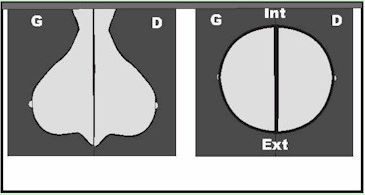
\includegraphics[scale=1.0]{images/mammogramMirror.png}
	\caption{A back to back position of the left and right breasts of both the MLO and CC views, Mammo}
  	\label{fig:mammogramMirror}
\end{figure}

	Masses are three-dimensional lesions in the sense that they're seen on multiple views. The location of a mass may be determined through the analysis of multiple views where observable masses are suspicious of malignancy. Size does not determine the malignancy of a mass, except if on successive views, the size of the mass regularly increases. Masses can be distinguished in five different types presented in figure \ref{fig:mammogramMassTypes}: round, oval, lobular, irregular, and architectural distortion  \cite{mammogramMass}.

\begin{figure}[h]
	\centering
  	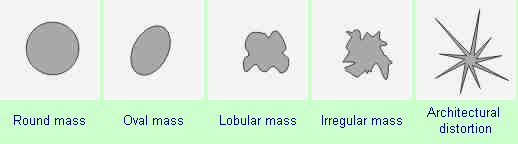
\includegraphics[scale=0.8]{images/mammogramMassTypes.png}
	 \caption{The five different types of mammogram masses, Mammo}
  	\label{fig:mammogramMassTypes}
\end{figure}

	Mass margins must also be detailed during analysis specifically the ROI they cover. As such, the five different margin types include circumscribed (well-defined and sharply demarcated), microlobulated (small circled line the edges), obscured, indistinct or ill-defined, and spiculated as seen in figure \ref{fig:mammogramMargin}. The obscured margins are due to adjacent normal tissue overlapping. Indistinct or spiculated margins illustrate the invasion of the malignant tumour into surrounding healthy tissue \cite{mammogramMass}.

\begin{figure}[h]
	\centering
  	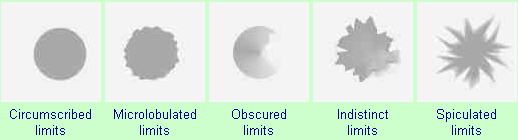
\includegraphics[scale=0.8]{images/mammogramMargin.png}
	 \caption{The five different types of mammogram mass margins, Mammo}
  	\label{fig:mammogramMargin}
\end{figure}

	 Generally, round, oval, or lobulated masses with circumscribed limits are benign tumors with only little known cases not following this rule \cite{regularBreastMasses}. Round masses with obscured limits are difficult to analyze often mimicking a cancer mass with ill-defined borders. In light of this, further breast examinations are performed. Masses with lobulated or microlobulated limits are suspicious of malignancy where the more lobulated the limits are, the greater the risk of malignancy. Masses with indistinct limits are also suspicious of malignancy \cite{irregularBreastMasses}. Masses observed as architectural distortions may also be a sign of malignancy, but they may also be a result of a surgical scar or unrelated diseases. Consequently, further breast examination must be performed. Masses with spiculated borders are highly suspicious of cancer as spicules illustrate invasion of the tumour into surrounding tissue \cite{irregularMasses}. \\

	Breast calcifications are small calcium deposits in women's breast tissue \cite{breastCalcification}. Calcification images should be detailed according to size, shape, number of calcifications, and distribution. Generally, larger calcifications (macrocalcifications) with regular or oval shapes are benign, while smaller, irregular calcifications (microcalcifications) are potentially malignant. Moreover, in analysing the size of calcifications, the sizes of microcalcification fall between 0.2 - 0.5 mm, while macrocalcification sizes are 2.0 mm or larger \cite{mammaryCalcifications}. \\

	When detailing the shape of calcifications, round, oval calcifications with uniform shape and size are suggestively benign, while irregular calcifications are potentially malignant. Furthermore, M. Le Gal proposed five types of microcalcifications according to shape with corresponding degrees of malignancy as detailed in figure \ref{fig:mammogramCalcificationTypes}: type I (tea-cup, annular, clear centres) with 0\% malignancy potential, type II (regularly punctiform) with 39\% malignancy potential, type III (dusty, salt particles) with 39\% malignancy potential, type IV (irregularly punctiform) with 59\% malignancy potential, and type V (vermicular punctiform) with 96\% malignancy potential \cite{mammaryCalcifications}.

\begin{figure}[h]
	\centering
  	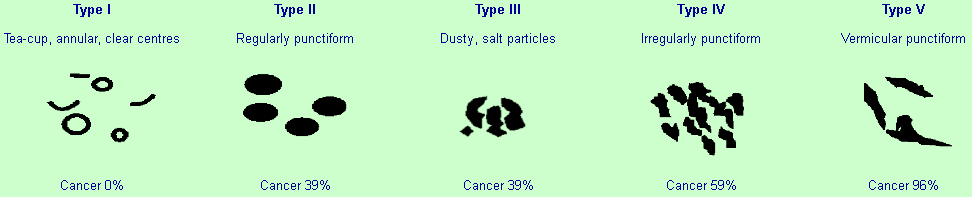
\includegraphics[scale=0.6]{images/mammogramCalcificationTypes.png}
	 \caption{The five different types of microcalcifications based on shape, Mammo}
  	\label{fig:mammogramCalcificationTypes}
\end{figure}

	Lastly, when analysing the number of calcifications, any number above four up to six microcalcifications is indicative of malignancy \cite{mammaryCalcifications}. \\

	After mammographic analysis and evaluation, the results are classified according to one of the following BI-RADS categories \cite{breastCancerScreeningAndDiagnosis}:

\begin{enumerate}
	\item{Category 0: Additonal imaging evaluation and/or comparison to prior mammograms is needed} \\
	The findings in the mammogram require additional imaging examination. Additional imaging examinations include ultrasound, MRI, special mammogram views, spot compression, and magnified views. Moreover, the mammogram of interest may be compared to past mammograms to identify changes over a period of time.

	\item{Category 1: Negative} \\
	The mammogram under study contain no significant abnormalities indicative of malignancy. The breasts appear healthy.

	\item{Category 2: Benign Findings} \\
	Like category 1, the mammogram of interest appear to contain no malignant abnormalities, but benign findings are present. Typical findings include benign-appearing macrocalcifications, oil cyst, or a lipoma.

	\item{Category 3: Probably Benign Findings; Short-Interval Follow-up Suggested} \\
	This is a mammogram that is usually benign, but further exploration should be performed to generate more stable readings.

	\item{Category 4: Suspicious Abnormality; Biopsy Should be Considered} \\
	The mammogram analyzed contains possible malignant abnormalities but not obviously malignant mammographically. A breast biopsy is recommended to verify malignancy.

	\item{Category 5: Highly Suggestive of Malignancy; Appropriate Action Should be Taken} \\
	The findings present in the mammogram are highly probable (> 95\%) of being malignant. Typical findings include spiculated mass or malignant-appearing microcalcifications. As such, breast biopsy is also recommended.

	\item{Category 6: Known Biopsy-Proven Malignancy; Appropriate Action Should be Taken} \\
	The findings on the mammogram have already been verified as malignant by a previous breast biopsy. This category is for mammograms that have cancer under study to see how well the cancer is responding to a particular treatment.
\end{enumerate}

\subsection{Machine Learning}

\qquad Machine learning is the science behind the ability of computers to act and learn concepts without being explicitly programmed, and improve learning over time through data and observations \cite{machineLearning}. To date, there are so many machine learning algorithms each with different uses for specific functions. Machine learning algorithms can be categorized into four types based on their purpose \cite{machineLearningTypes}:

\begin{enumerate}
	\item{Supervised Learning} \\
	In supervised learning problems, a data set is procured containing training examples or instances with associated correct labels or predictions. For example, the problem is to have the computer learn to classify handwritten digits. In a supervised learning approach, a data set must be acquired with thousands of pictures of handwritten digits along with labels identifying the correct number illustrated by image. The implemented algorithm would attempt to learn and acquire features from the images with respect to the number they represent in order to build a model to classify said images. The model would undergo several parameter tweakings and adjustments to achieve an optimal model. This process is referred to as training. Then, the model would be put to the test to classify handwritten digits on an unlabeled data set \cite{supervisedLearning}. Algorithms under supervised learning include Nearest Neighbor, Naive Bayes, Deision Trees, Linear Regression, Support Vector Machines (SVM), and Neural Networks.

	\item{Unsupervised Learning} \\
	In contrast to supervised learning, unsupervised learning involves training the computer with unlabeled data. This type of machine learning is typically used for pattern detection and descriptive modeling. Since there are no labels for which an algorithm can model relationships, unsupervised learning algorithms attempt to utilize techniques on the data to mine for rules, detect patterns, and summarize and group the data. Some common algorithms include k-means clustering and Association Rules.

	\item{Semi-supervised Learning} \\
	Semi-supervised learning involves a combination of the first two types. In order for supervised learning to be at its most effective, a large labeled data set is required. However, in practical situations, the cost of labeling is high, and, in some fields, a large fully-labeled data set lacks. So, in the absence of correct labels in the majority of the observations but present in few, semi-supervised learning algorithms may be implemented.
\end{enumerate}

	Furthermore, there are algorithms centered on a specific technique of machine learning called deep learning (DL). The main advantage of DL algorithms over ML algorithms is that DL algorithms can generate new features from existing ones in the training data set, while in ML algorithms, the features must be accurately identified which can be costly. Therefore, DL algorithms save more time when dealing with large, big complex data \cite{advantageDeepLearning}. \\

	Artificial neural networks (ANN), inspired by the biological structure of the human brain, are machine learning algorithms applied on the computer to perform specific tasks such as clustering, classification, pattern recognition, etc. A typical ANN contains hundreds of interconnected single units, artificial neurons, connected with coefficients (weights), which constitute the neural structure and are grouped and separated in layers. The behavior of an ANN depends on several factors such as the activation function of a neuron, the weights of each neuron, biases of each layer, the learning rule of the ANN, the architecture itself, etc. The output of a single neuron is determined by the weighted sum of the inputs passed through the activation function \cite{artificialNeuralNetworks}. \\

	During training, the training set is passed through the network, and the output obtained is compared with the actual value. The difference between the predicted output and the actual value is referred to as the error. The objective of training the network is to achieve a model where the parameters are optimized in such a way that the error in predictions is minimized specifically the error converges to a local minimum \cite{artificialNeuralNetworks}. \\

\subsection{Convolutional Neural Networks}
\qquad Convolutional Neural Network (CNN) is a common DL algorithm and a special case of ANNs. Historically, CNNs are mainly used for image recognition tasks specifically object detection and classification, due to their ability to learn higher-order features. A CNN is primarily composed of one or more convoluational and pooling (or subsampling) layers and then followed by one or more fully-connected layers. Figure \ref{fig:CNN} illustrates how a standard CNN architecture handles a vehicle image classification task. An image is input into the network where it undergoes several stages of convolution and pooling. The features extracted from the process are fed into the fully-connected neural network. Finally, the last fully-connected neural network outputs the predicted classification \cite{convolutionalNeuralNetworks}.

\begin{figure}[h]
	\centering
  	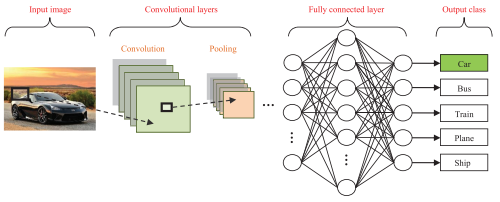
\includegraphics[scale=1.0]{images/CNN.png}
	 \caption{An intuitive overview of a standard CNN, Mammo}
  	\label{fig:CNN}
\end{figure}

	In the convolutional layer, features are extracted, and the feature representations of the input image is obtained. The convolutional layer's parameters involves a set of learnable filters typically small in dimension but extends through the full depth of the input volume (i.e. a filter for the first layer of size 5x5x3, with 5x5 height and witdth, and depth 3 for color channels). In the processing of the input volume, the filter slides (convolves) across the width and height of the input volume, while dot products are computed from the filter entries and the input. Typically, the first convolutional layers learn low-level features like edges or blotches of some color, while the latter layers learn higher level features \cite{convolutionalLayers}. Figure \ref{fig:convolutionalLayer} illustrates how convolution works. \\

\begin{figure}[h]
	\centering
  	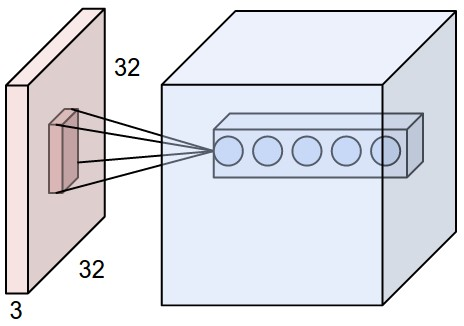
\includegraphics[scale=0.5]{images/convolutionalLayer.jpeg}
	 \caption{An illustration of an input volume (i.e. 32x32x3 input image) at the left and the first convolutional layer (a volume of neurons) to the right; image, Mammo}
  	\label{fig:convolutionalLayer}
\end{figure}

	The pooling layer, commonly placed in succession with several convolutional layers, serves to progressively reduce the spatial size of the representation in order to reduce the amount of parameters and computational costs in the network. There are two types of pooling namely average pooling and max pooling. Figure \ref{fig:poolingLayer} illustrates the difference between the two types \cite{convolutionalNeuralNetworks}. \\

\begin{figure}[h]
	\centering
  	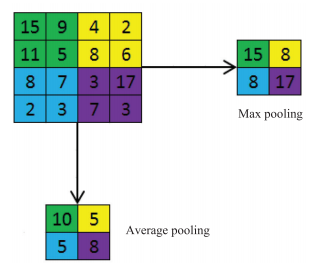
\includegraphics[scale=0.8]{images/poolingLayer.png}
	 \caption{Average pooling vs max pooling, Mammo}
  	\label{fig:poolingLayer}
\end{figure}

	In figure \ref{fig:poolingLayer}, a common pooling layer form is used where the filter size is 2x2 applied with a stride of 2. The input image here has a size of 4x4. After pooling is applied, max pooling outputs the maximum value of each 2x2 region, while average pooling outputs the average of each region. \\

	Lastly, the fully-connected layers interpret the feature representations extracted from the convolutional and pooling layers in order to arrive at a conclusion. The last layer here outputs the predicted class label.

\subsection{Residual Neural Networks}
\qquad According to He et. al \cite{Resnet}, the motivation behind Residual Neural Networks (ResNet) is a property of CNNs: as more layers are stacked (as the CNN goes deeper), the levels of features integrated by the network are enriched which would entail better model generalization. However, as a CNN goes deeper, the network becomes more difficult to train due to the problem of vanishing and exploding gradients. Moreover, when deeper networks are able to start converging, a degradation problem occurs where, due to the increase in network depth, the accuracy becomes saturated and then degrades rapidly resulting to higher training error. \\

	In their study \cite{Resnet}, the authors attempt to address the degradation problem by introducing a deep residual learning framework. In their network, instead of having some stacked layers fit a desired underlying mapping, they let the stacked layers fit a residual mapping. The authors have hypothesized that it is easier to optimize the residual mapping than to optimize the underlying, original mapping. The construction of such residual mapping can be realized by CNNs with "shortcut connections." Shortcut connections are those skipping one or more layers through the use of identity mapping, where the outputs are added to the outputs of the stacked layers as seen in figure \ref{fig:resNetSample}. \\

\begin{figure}[h]
	\centering
  	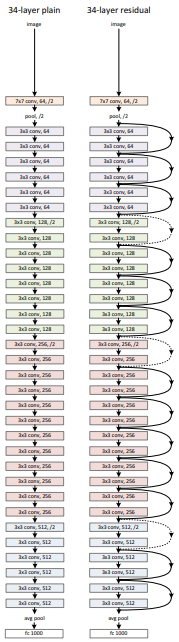
\includegraphics[scale=0.8]{images/resnet.png}
	 \caption{Left: a plain CNN with 34 parameter layers. Right: a RNN with 34 parameter layers. The dotted shortcuts increase dimensions, Mammo}.
  	\label{fig:resNetSample}
\end{figure}

	The authors have provided comprehensive evidence that their proposed residual learning framework is effective as they've obtained excellent results on the ImageNet classification data set with their 152-layer RNN where they obtained a 3.57\% top-5 error, and won 1st place in the ILSVRC 2015. \\

	As stated, the network architecture used is a pretrained ResNet-50 which is a ResNet with 50 parameter layers.
\clearpage
\section{Design and Implementation}

\subsection{System Overview}
\begin{figure}[h]
	\centering
  	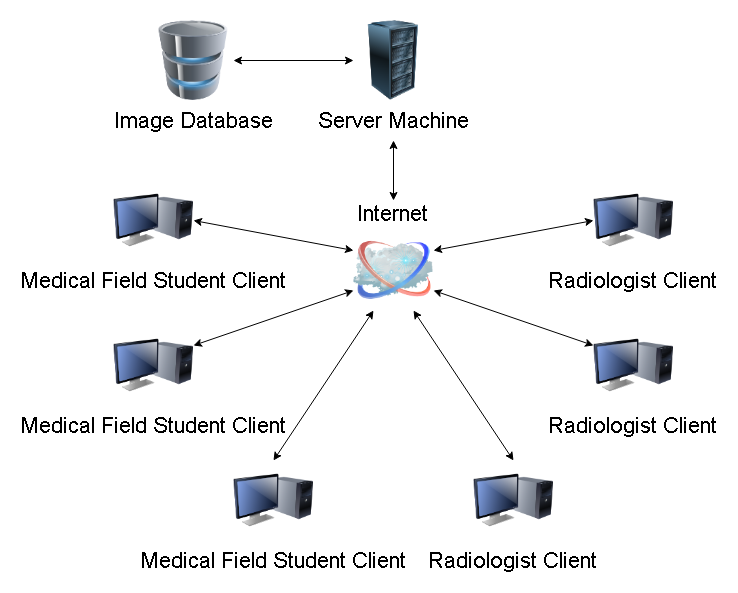
\includegraphics[scale=0.5]{images/systemOverview.png}
	 \caption{System Overview, Mammo}
  	\label{fig:systemOverview}
\end{figure}

	The Decision Support System includes a typical client-server architecture. The client sends requests to the server. The server processes the client's request. There are two types of clients namely the Medical Field Student Client (MFSC) and the Radiologist Client (RC). The MFSC and the RC can send mammogram images through desktop computers for evaluation to the server by which the server, in turn, returns the results. The MFSC may also request for an exam, and the server redirects the MFSC to the exam proper.
\clearpage

\subsection{Use Case Diagram}
\qquad Figure \ref{fig:useCase} shows the general functionalities of each user. Both the Medical Field Student and Radiologist have the functionality of uploading a mammogram image for the system to classify whether benign or malignant, and retrieving the classification result. The Medical Field Student also has the option to take an exam on screening mammograms.

\begin{figure}[!htb]
	\centering
  	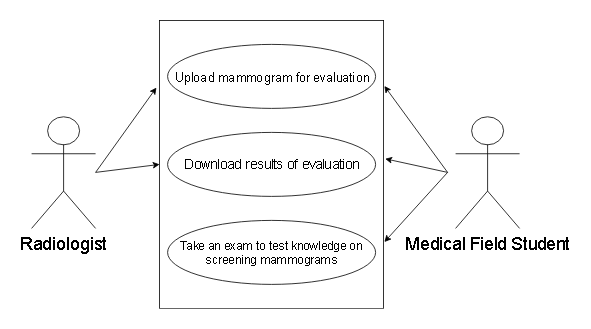
\includegraphics[scale=0.8]{images/useCase.png}
	 \caption{Use Case Diagram, Mammo}
  	\label{fig:useCase}
\end{figure}
\clearpage


\subsection{Activity Diagram}

\begin{enumerate}
	\item{Radiologist} \\
	The radiologist can also send a mammgram image for evaluation using the web application.

\begin{figure}[h]
	\centering
  	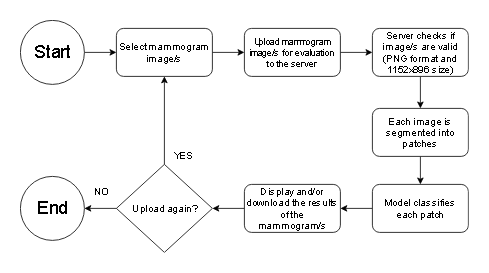
\includegraphics[scale=0.75]{images/radiologist.png}
	 \caption{Radiologist Activity Diagram, Mammo}
  	\label{fig:radiologist}
\end{figure}
\clearpage

	\item{Medical Field Student} \\
	The medical field student can send a mammogram image for evaluation using the web application. The medical field student may also request for an exam on screening mammograms. The results of the exam are given immediately after.

\begin{figure}[h]
	\centering
  	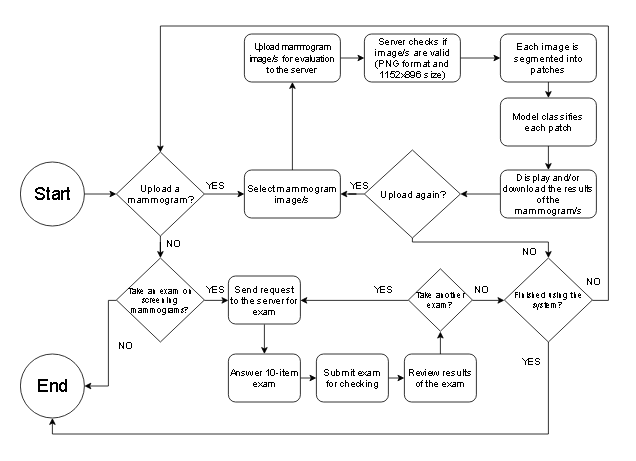
\includegraphics[scale=0.75]{images/medicalFieldStudent.png}
	 \caption{Medical Field Student Activity Diagram, Mammo}
  	\label{fig:medicalFieldStudent}
\end{figure}
\end{enumerate}
\clearpage

\subsection{Technical Architecture}
\qquad The recommended requirements for the server machine include:

\begin{itemize}
	\item 2 GHz CPU rate or higher
	\item Graphics Processing Unit (GPU) specifically a NVIDIA Graphics Card with 3.0 compute capability or higher
	\item 8 GB RAM or higher
	\item Up to 2 GB of free disk space
\end{itemize}

	The client side must have any of the following compatible up-to-date web browsers:

\begin{itemize}
	\item Google Chrome
	\item Mozilla Firefox
	\item Safari
\end{itemize}

\subsection{Data Set}
\qquad The data set used is the CBIS-DDSM (Curated Breast Imaging Subset of the Digital Database for Screening Mammography) which is an updated and standardized version of the DDSM \cite{CBIS-DDSM}. The data set contains 2583 cropped mammogram ROI images in DICOM format of 1249 patients labeled as benign or malignant cases with verified pathology information. It includes the CC and MLO views for most of the screened breasts. The data set is publicly available through TCIA (The Cancer Imaging Archive) which is an online service that hosts a large archive of medical images of cancer accessible for public download \cite{TCIA}.
\section{Results}

\subsection*{Training the Convolutional Neural Network}
\qquad The dataset, CBIS-DDSM (Curated Breast Imaging Subset of the Digital Database for Screening Mammography), was downloaded from TCIA (The Cancer Imaging Archive). The dataset downloaded was similar to that in Shen's study \cite{CNNmodel}. But, instead of the whole-image dataset version of CBIS-DDSM, the dataset downloaded was the cropped region of interest (ROI) version.

\subsubsection{Preparing the Dataset}
\qquad Preparing the dataset was no easy task, for the dataset was erroneous. For context, there are two file locations in the given CSV metadata file for the whole dataset: one for the cropped ROI, and the other for the ROI mask. There are several occurences where the file location of the cropped ROI was mislabeled and would point to the ROI mask instead. Since there are several occurences in the dataset's metadata where file locations are erroneous, there is no way of confirming if the other information are erroneous as well. This poses a potential problem where the ROIs are misclassified. It is this for this reason that the erroneous instances are kept track of.
	
\subsubsection{Setting the Hyperparameters}	
\qquad After setting the proper number of epochs, learning rate, batch size, and the optimizer namely Nesterov Gradient Descent seen in figure \ref{fig:hyperparameters} as well as utilizing a pre-trained ResNet-50 model, and having the model undergo initial training, the model looked promising as it slowly converges shown in figure \ref{fig:firstModelLog1} for the first few iterations and figure \ref{fig:firstModelLog2} for the last remaining iterations. However, after having the model tested, it only attained an accuracy of 33\% as it correctly labeled 243 images from a test set of 704. A possible cause for such a low accuracy is the lack of data augmentation techniques applied on the dataset used. Another cause is the imbalanced number of instances per category specifically there are 681 ROI images for benign mass, 637 ROI images for malignant mass, 1,002 ROI images for benign calcification, and 544 ROI images for malignant calcification.

\begin{figure}[h]
	\centering
  	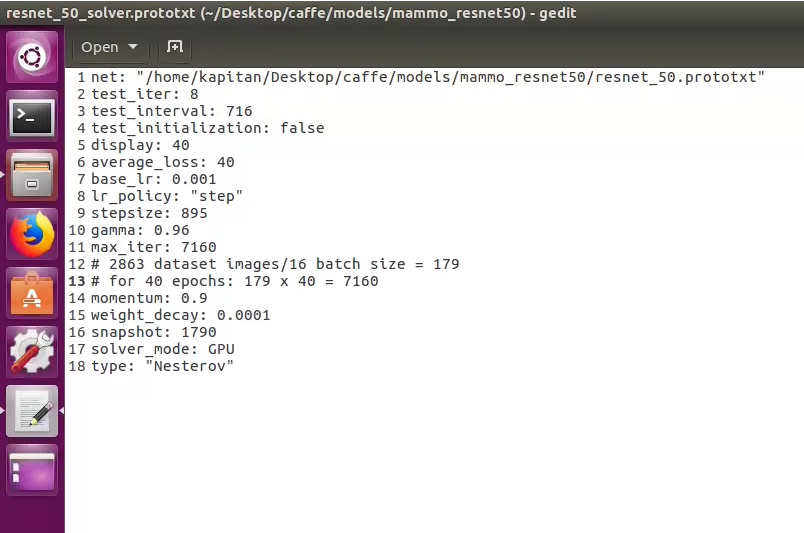
\includegraphics[scale=0.6]{images/hyperparameters.png}
	\caption{ResNet-50's hyperparameters, Mammo}
  	\label{fig:hyperparameters}
\end{figure}

\begin{figure}[h]
	\centering
  	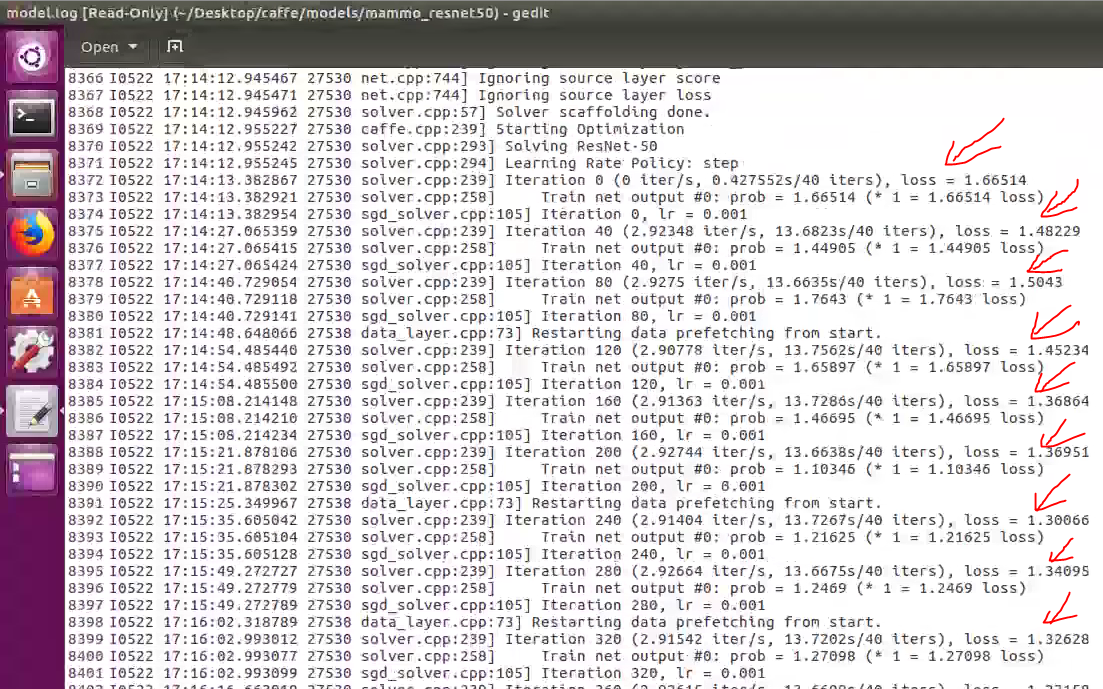
\includegraphics[scale=0.5]{images/firstModelLog.png}
	\caption{The log file of the model showing diminishing loss on the first few iterations as indicated by the red arrows, Mammo}
  	\label{fig:firstModelLog1}
\end{figure}

\begin{figure}[h]
	\centering
  	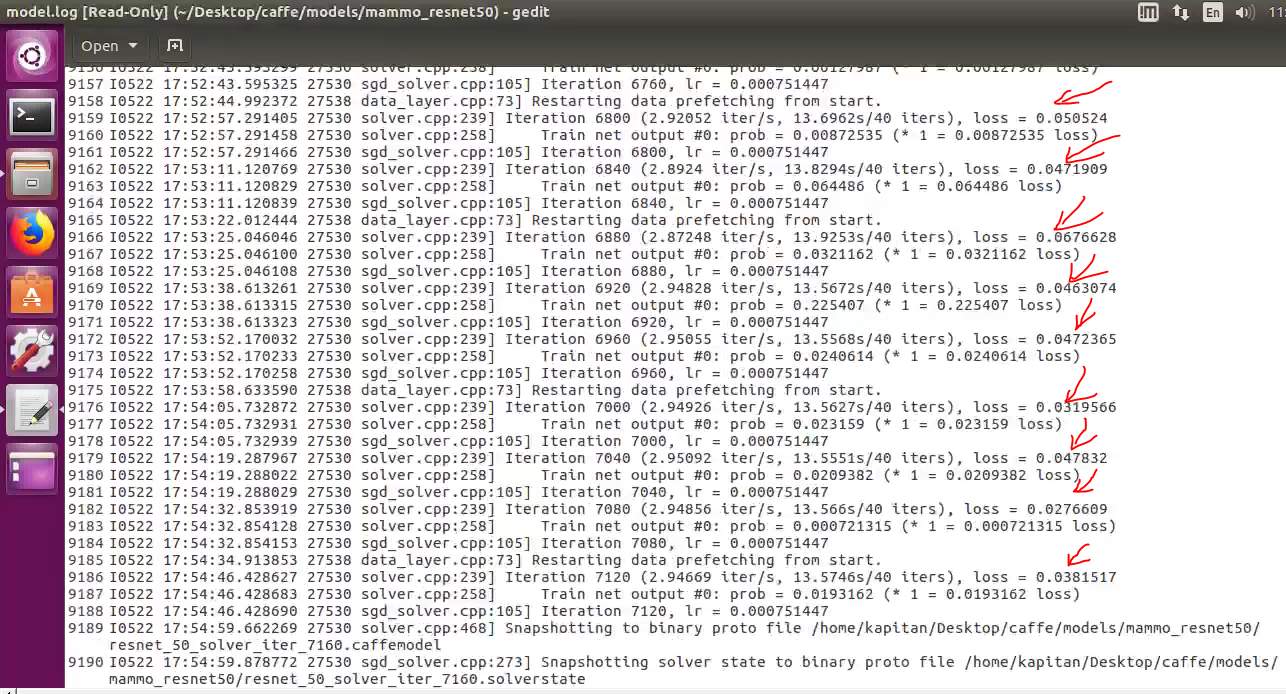
\includegraphics[scale=0.5]{images/firstModelLog2.png}
	\caption{The log file of the model showing diminishing loss on the last remaining iterations as indicated by the red arrows, Mammo}
  	\label{fig:firstModelLog2}
\end{figure}

\subsubsection{Improving the Accuracy}
\qquad To address the low accuracy, the dataset was balanced having the number of images under each category set at a maximum of 544 ROI images. This was done by removing the extra erroneous instances from each category, and then randomly removing other ones until it reached 544 images except images under malignant calcification. Then the model was trained again with the same hyperparameters except for the number of epochs which was increased from 40 to 50, and the use of the balanced dataset. Figures \ref{fig:secondModelLog1} and \ref{fig:secondModelLog2} show the model's convergence at the first few iterations, and at the last remaining iterations. The accuracy improved up to 43\% with the model correctly classifying 305 images out of 704 as seen in figure \ref{fig:secondModelAccuracy}.

\begin{figure}[h]
	\centering
  	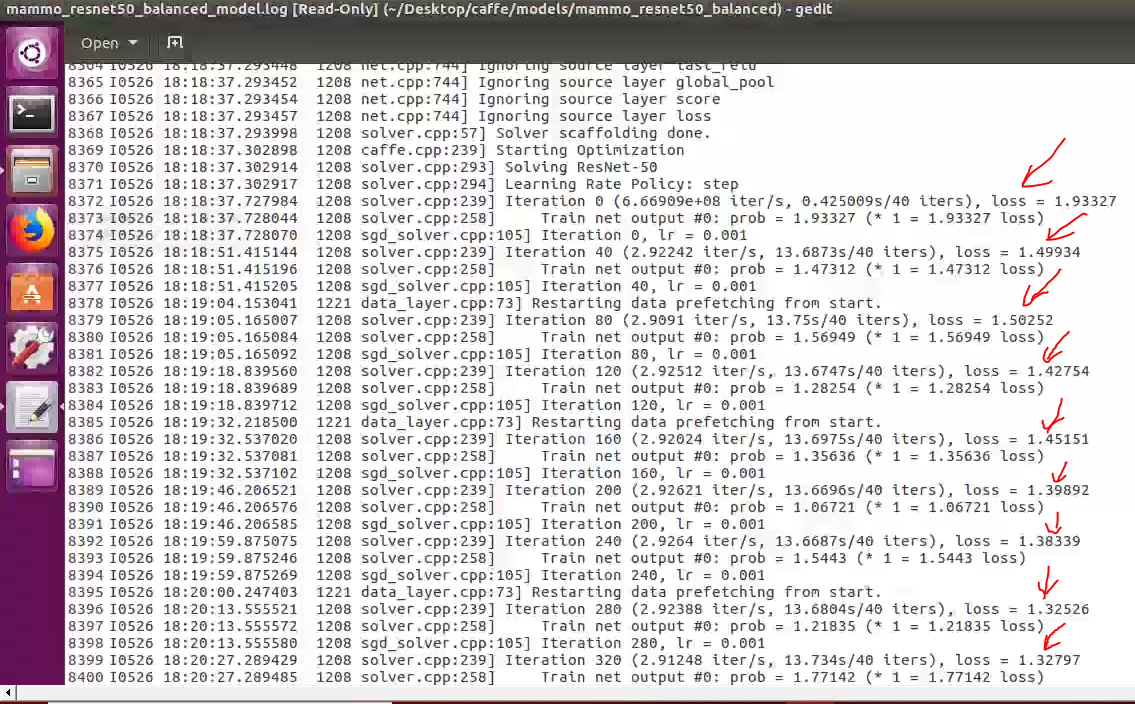
\includegraphics[scale=0.5]{images/secondModelLog.png}
	\caption{The log file of the model with the balanced dataset diminishing improving loss on the first few iterations as indicated by the red arrows, Mammo}
  	\label{fig:secondModelLog1}
\end{figure}

\begin{figure}[h]
	\centering
  	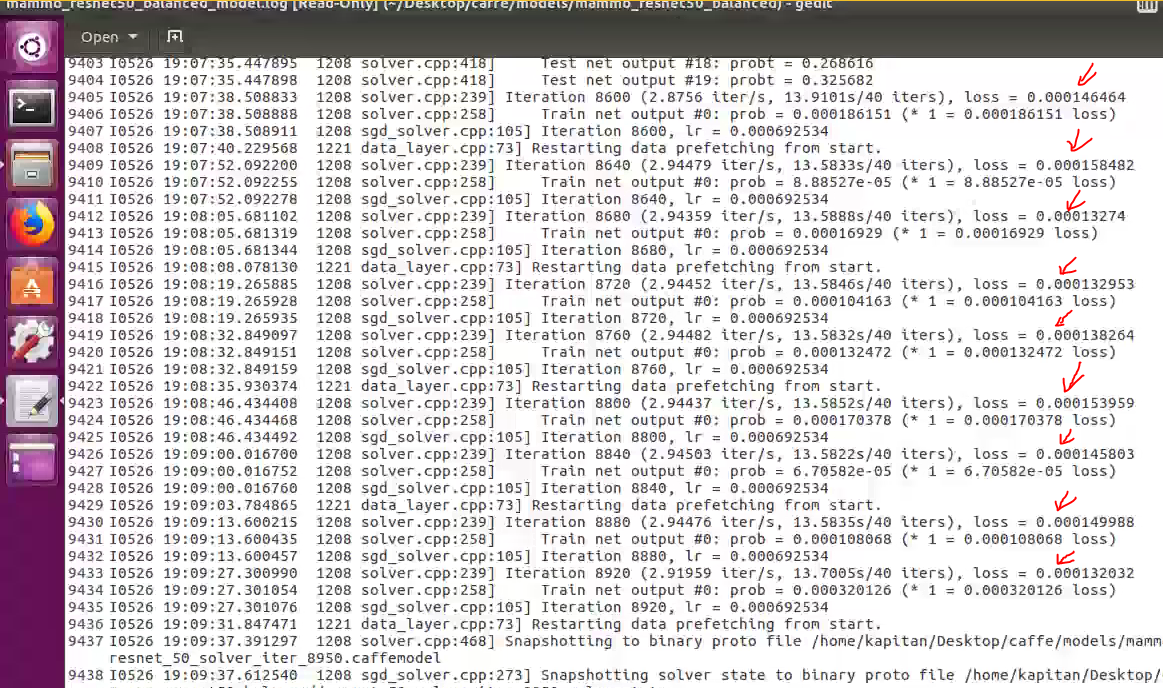
\includegraphics[scale=0.5]{images/secondModelLog2.png}
	\caption{The log file of the model with the balanced dataset diminishing improving loss on the last remaining iterations as indicated by the red arrows, Mammo}
  	\label{fig:secondModelLog2}
\end{figure}

\begin{figure}[h]
	\centering
  	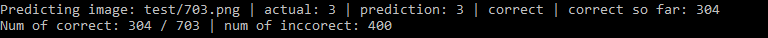
\includegraphics[scale=0.5]{images/secondModelAccuracy.png}
	\caption{The accuracy of the model after balancing the dataset, Mammo}
  	\label{fig:secondModelAccuracy}
\end{figure}
	
\subsection*{General User Functionalities}
\qquad The home page of the system is seen in  figure \ref{fig:mammoHome}. A basic description of what the site is for is present here along with the features it has to offer. Also, a navbar that provides the user access to the site's features is present at all pages of the site.

\begin{figure}[h]
	\centering
  	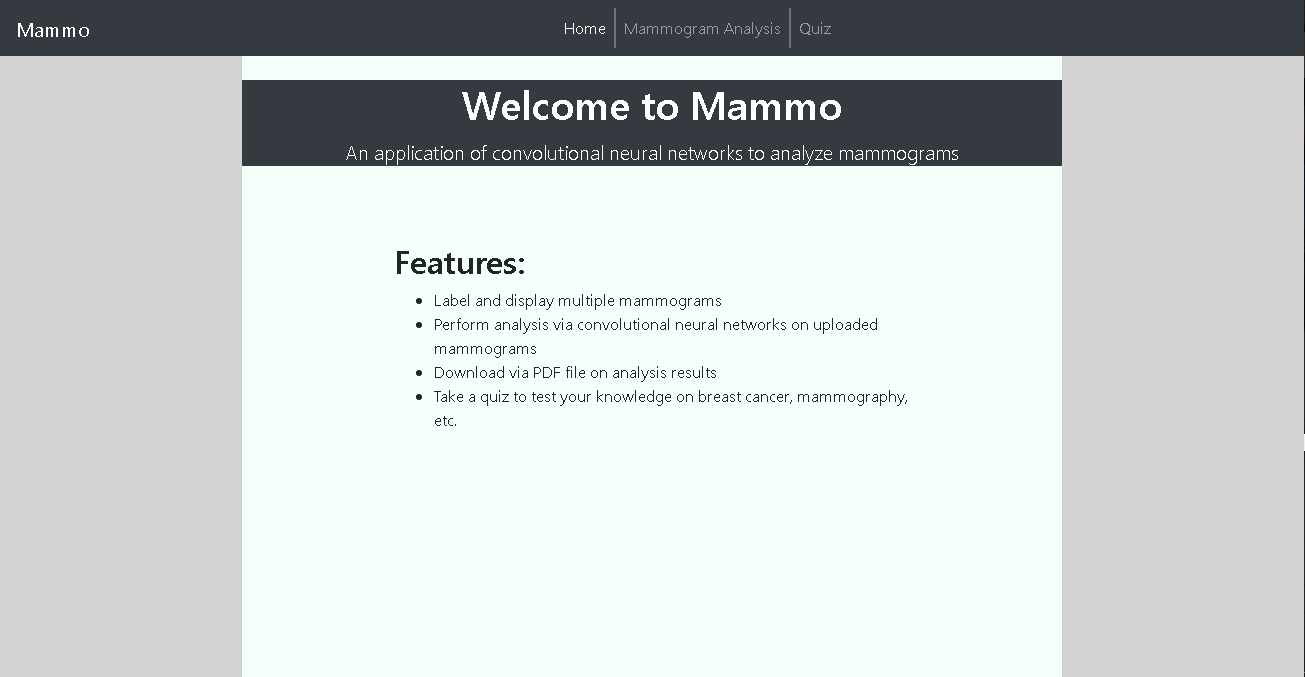
\includegraphics[scale=0.5]{images/mammoHome.png}
	\caption{Mammo home page, Mammo}
  	\label{fig:mammoHome}
\end{figure}

\subsection{Mammogram Analysis}

\subsubsection{Uploading Mammograms}
\qquad Figure \ref{fig:uploadMammograms} shows that a user has fully uploaded his chosen mammograms. A user may do this through the "Add Images" button at the top of the left sidebar or by just dragging and dropping files from his/her directory.

\begin{figure}[h]
	\centering
  	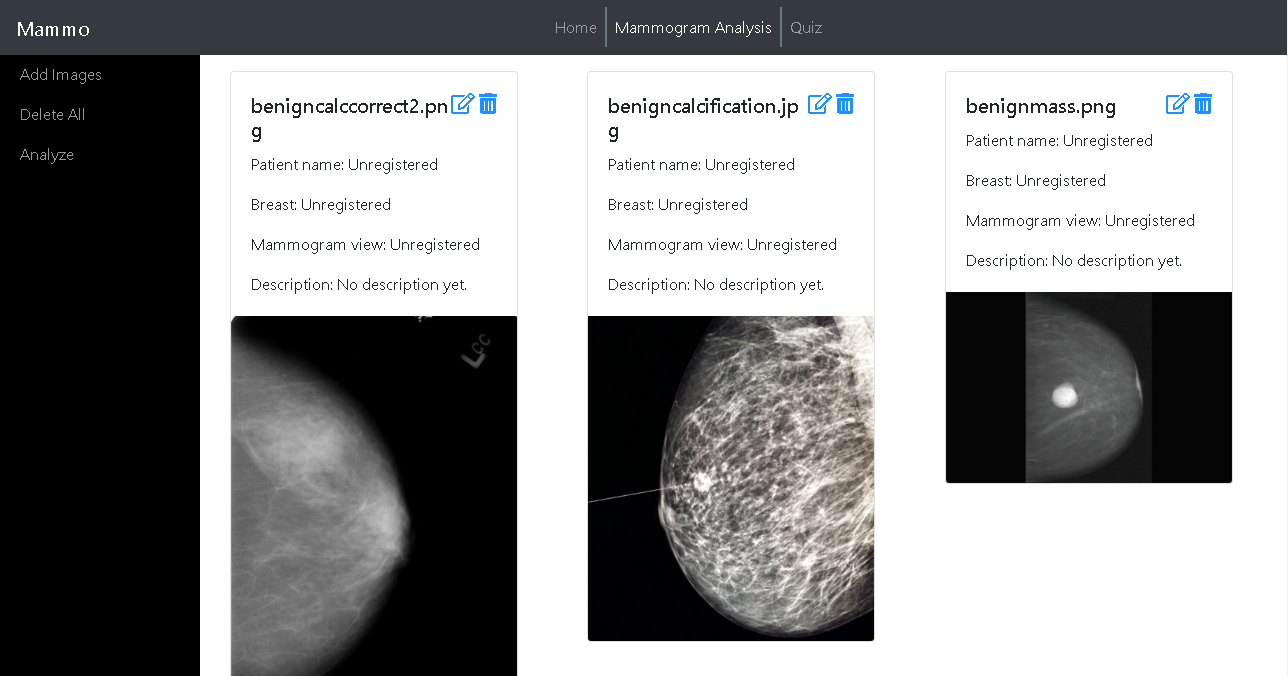
\includegraphics[scale=0.5]{images/uploadMammograms.png}
	 \caption{Three uploaded mammograms, Mammo}
  	\label{fig:uploadMammograms}
\end{figure}

\subsubsection{Editing and Deleting Mammograms}
	\qquad The mammograms are uploaded with unregistered metadata that is up for the user to edit. A user may edit the mammograms by clicking the edit icon present at the upper right of the mammogram cards, or he may simple click on the picture of the mammogram as shown figure \ref{fig:editMammograms}. Also, a user may delete the mammogram by pressing the delete icon next to the edit. Moreover, a user may delete all the mammograms uploaded by the "Delete All" button on the sidebar. Also, a user must specify the region of interest to be analyzed by the CNN module. A user may leave the metadata entries blank, but he must choose a region of interest and save it.

\begin{figure}[h]
	\centering
  	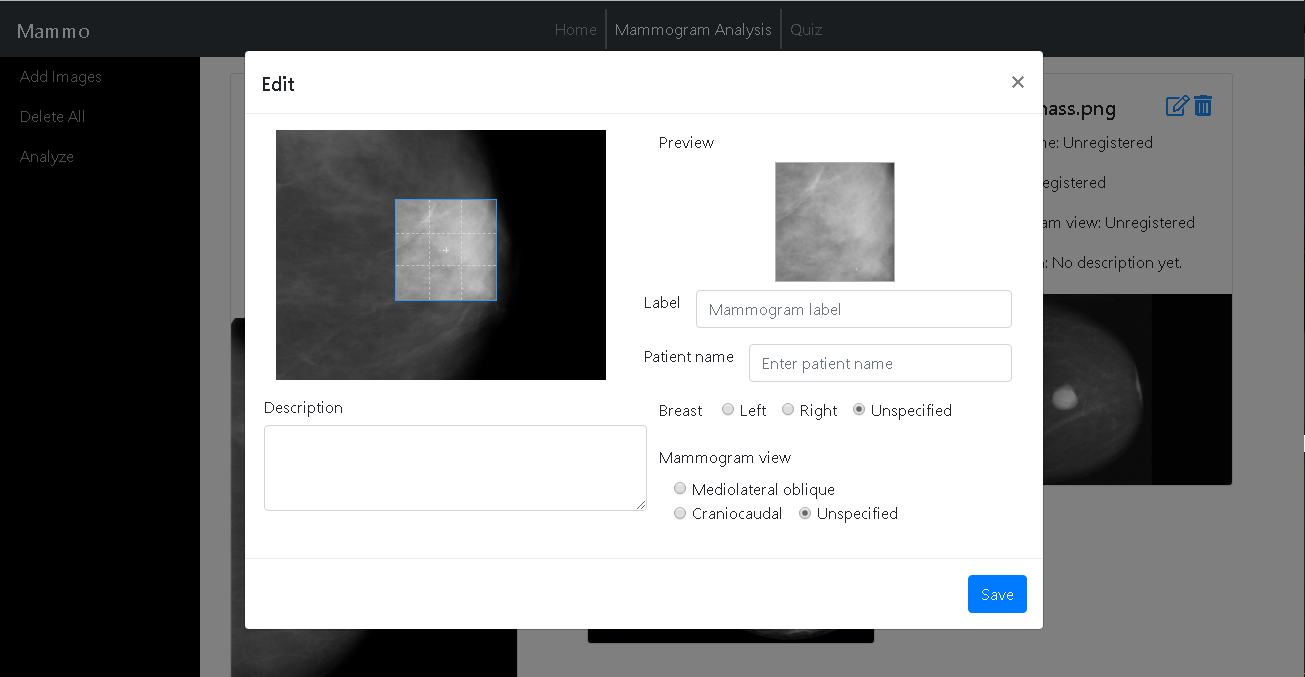
\includegraphics[scale=0.5]{images/editMammograms.png}
	 \caption{Editing metadata of the mammogram, Mammo}
  	\label{fig:editMammograms}
\end{figure}


\subsubsection{Analyzing the Mammograms}
	\qquad After the user has entered the necessary patient data, he/she may then proceed to have the mammograms analyzed by the "Analyze Mammograms" on the sidebar (see figure \ref{fig:uploadMammograms}). It may take a long time to process the mammograms. Figures \ref{fig:mammogramAnalysis1} and \ref{fig:mammogramAnalysis2} show the analysis made by the CNN module. A "Generate PDF" functionality is present for the user to save the results as PDF (see figure \ref{fig:mammogramPDF}).

\begin{figure}[h]
	\centering
  	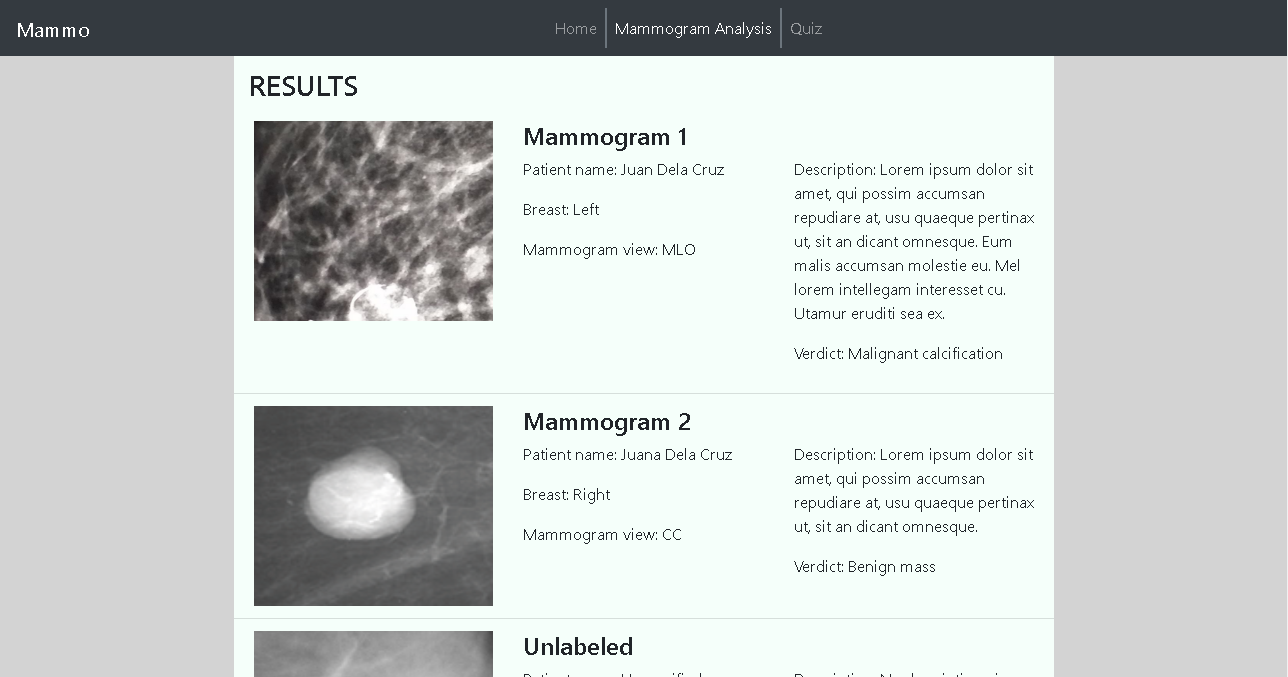
\includegraphics[scale=0.5]{images/mammoAnalysis1.png}
	 \caption{Results of the analysis made by the CNN module part 1, Mammo}
  	\label{fig:mammogramAnalysis1}
\end{figure}

\begin{figure}[h]
	\centering
  	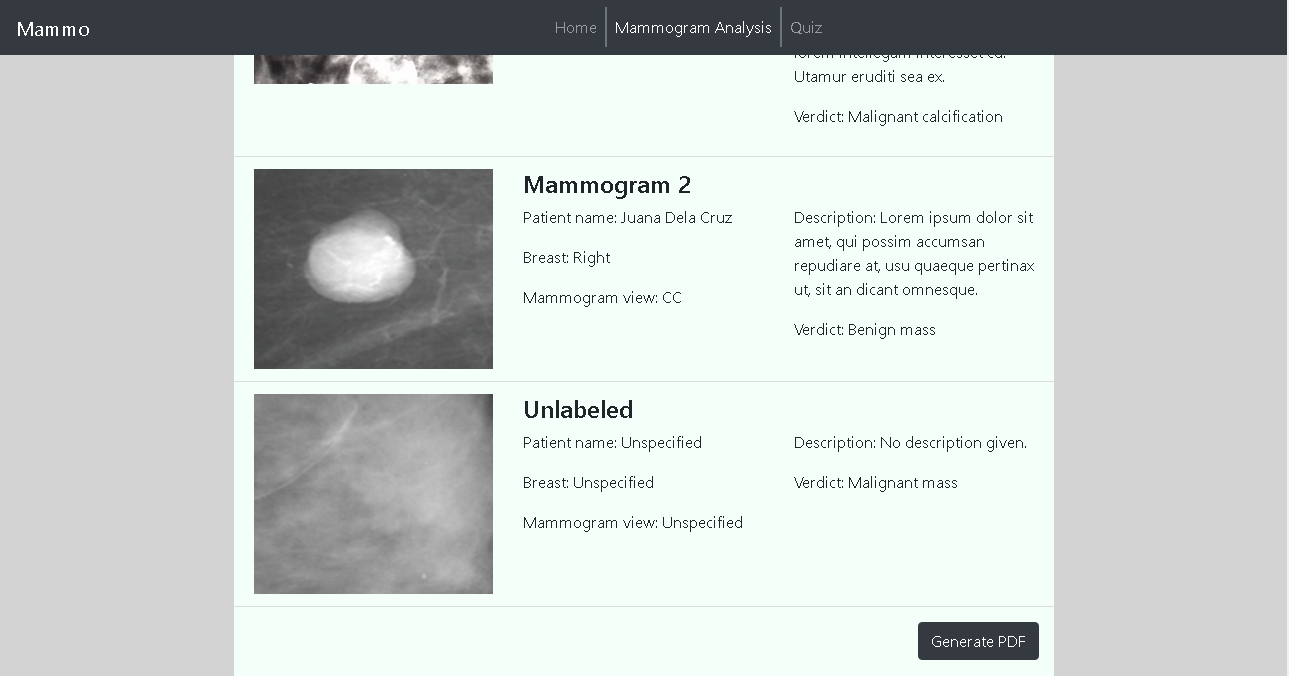
\includegraphics[scale=0.5]{images/mammoAnalysis2.png}
	 \caption{Results of the analysis made by the CNN module part 2, Mammo}
  	\label{fig:mammogramAnalysis2}
\end{figure}

\begin{figure}[h]
	\centering
  	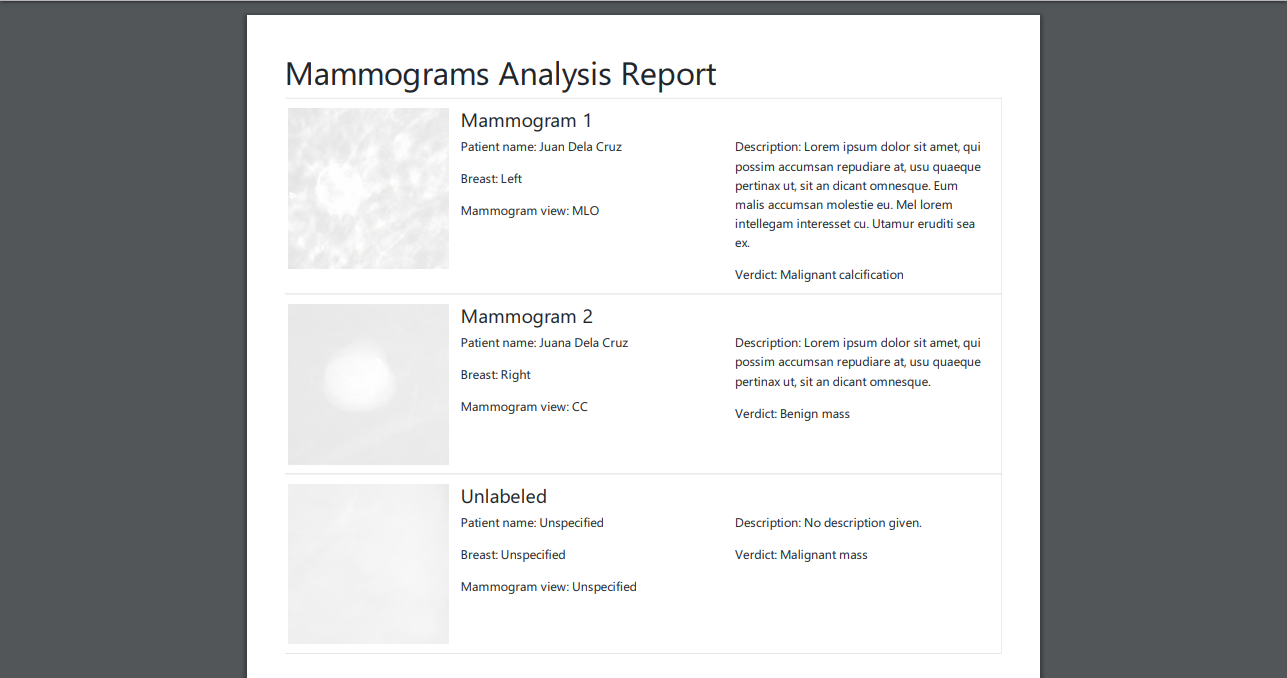
\includegraphics[scale=0.5]{images/mammogramPDF.png}
	 \caption{A generated PDF file of Mammogram Analysis Report, Mammo}
  	\label{fig:mammogramPDF}
\end{figure}

\subsection{Quiz}

\subsubsection{Taking the Quiz}
\qquad A user or a student/trainee has the option to take a randomly-generated 10-item pop quiz regarding breast cancer, mammography, treatment, etc. (see figure \ref{fig:mammogramExam}).

\begin{figure}[h]
	\centering
  	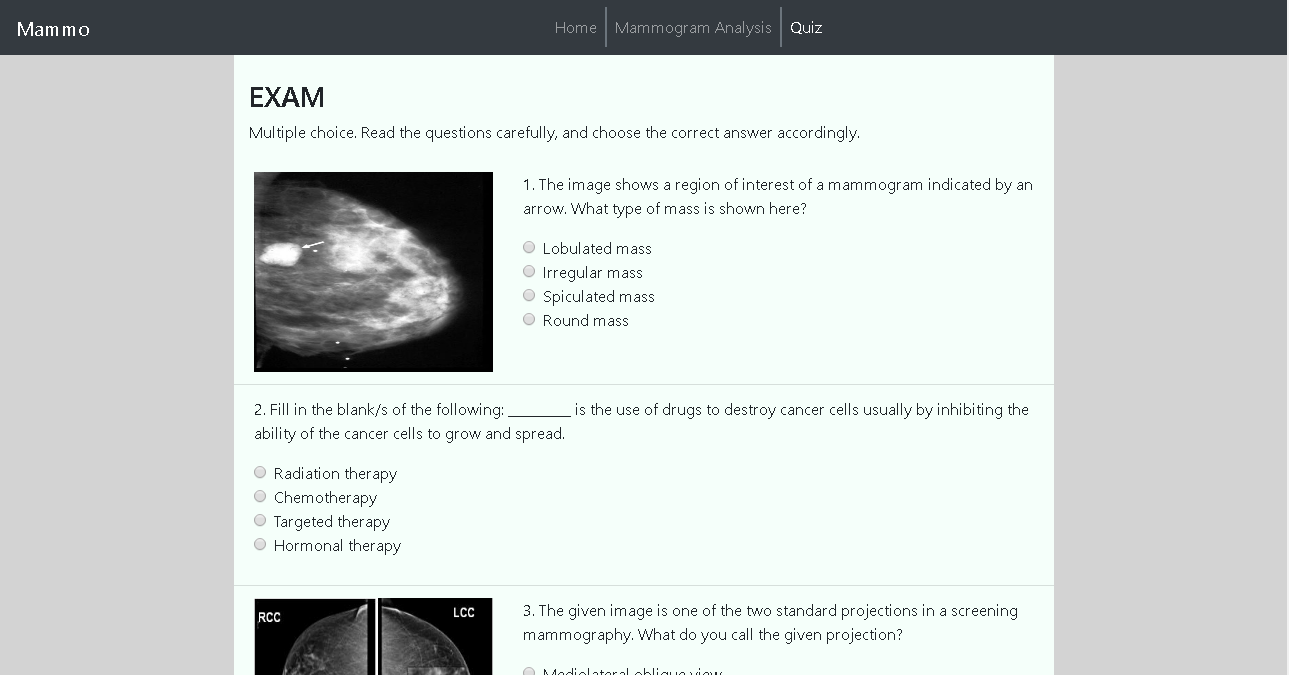
\includegraphics[scale=0.5]{images/mammogramExam.png}
	 \caption{A sample of the quiz, Mammo}
  	\label{fig:mammogramExam}
\end{figure}

\subsubsection{Quiz Results}
\qquad After the user has answered the questions and reviewed the answers, he/she may submit the quiz for evaluation by the "Submit" button seen in figure \ref{fig:submitQuiz}. The user's score and the correct answer are seen in figure \ref{fig:quizResults}.

\begin{figure}[h]
	\centering
  	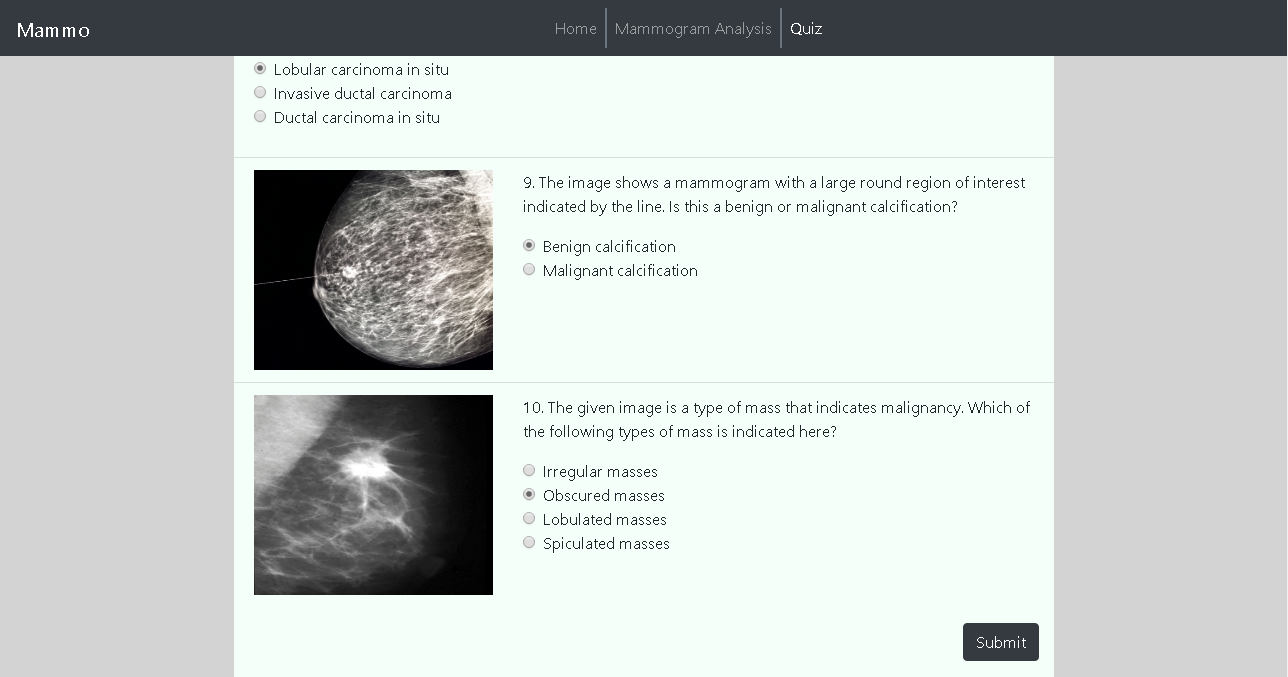
\includegraphics[scale=0.5]{images/submitQuiz.png}
	 \caption{Submit the quiz, Mammo}
  	\label{fig:submitQuiz}
\end{figure}

\begin{figure}[h]
	\centering
  	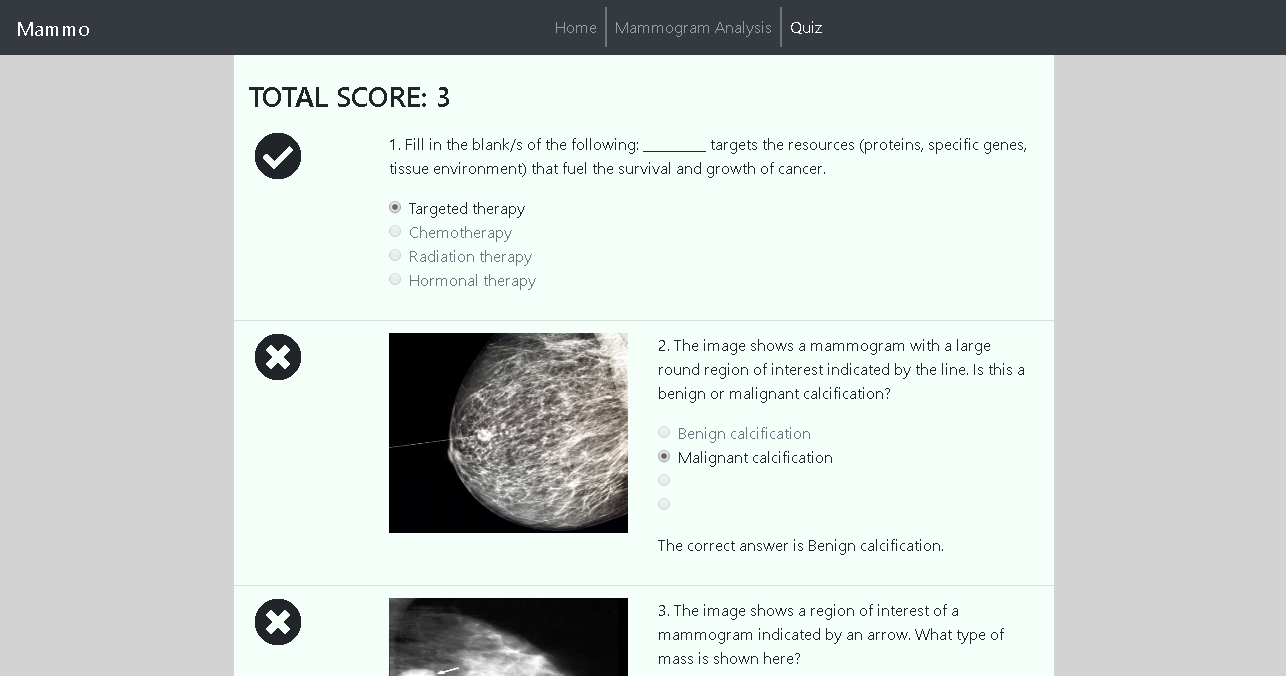
\includegraphics[scale=0.5]{images/quizResults.png}
	 \caption{Results of the quiz, Mammo}
  	\label{fig:quizResults}
\end{figure}

\clearpage
\clearpage
\section{Discussion}
\qquad Mammo is developed using a Convolutional Neural Network (CNN) specifically a Residual Neural Network with 50 layers which aims to assist radiologists, medical students and trainees to classify four breast lesions seen in mammography. It assists in classifying benign mass, malignant mass, benign calcification, and malignant calcification. The users have the functionality of uploading a mammogram, then choosing a region of interest for cropping and analysis by the model. The users also have the functionality of taking an exam in breast cancer, mammography, and other related topics. \\

	The rationale behind having the user choose and crop a ROI from a mammogram is because the CNN model is purely trained on cropped ROIs of mammograms. Moreover, the model was trained in this manner because the ROIs have more distinct features for the model to work with when compared to their whole image counterparts \cite{CNNmodel}. \\

	The model was trained on CBIS-DDSM (Curated Breast Imaging Subset of the Digital Database for Screening Mammography). But, as stated before, the dataset was erroneous.There are several occurences in the dataset's metadata where file locations are erroneous, so there is no way of confirming if the other information are erroneous as well. The proper measure was to clean the dataset by keeping track of the erroneous instances, and removing them from the dataset. This is because having a model trained under misclassified data would be problematic to the model's generalization. After the dataset has been cleaned, the images were converted from DICOM to PNG. \\

	The hyperparameters of the model was set in the following manner: the number of epochs set to 40, the base learning rate set to 0.001, the batch size set to 179, and the optimizer set to Nesterov Gradient Descent. Initially, the optimizer was set to Stochastic Gradient Descent, but the model did not converge whereas when the optimizer was set to Nesterov Gradient Descent, the model slowly converged as indicated in the model's log file. However, after having the model tested, it only attained an accuracy of 33\% as it correctly labeled 243 images from a test set of 704. A possible cause for such a low accuracy is the lack of data augmentation techniques applied on the dataset used, for these are known to improve accuracy \cite{araujo}. Another cause is the imbalanced number of instances per category specifically there are 681 ROI images for benign mass, 637 ROI images for malignant mass, 1,002 ROI images for benign calcification, and 544 ROI images for malignant calcification. \\

	To address the low accuracy, the dataset was balanced having the number of images under each category set at a maximum of 544 ROI images. This was done by randomly removing extra images from each category until it reached 544 images except images under malignant calcification. Then the model was trained again with the same specifications, and the use of the balanced dataset. The accuracy improved up to 43\% with the model correctly classifying 305 images out of 704. \\

	In comparison with Shen's ResNet-50 model \cite{CNNmodel}, the two networks are similar in terms of the architecture, and the dataset used. However, Shen utilized the whole-image version of the dataset while this study utilized the cropped region of interest (ROI) version of the dataset. Another notable difference was that Shen extracted the ROI from each of the whole images in the dataset and made a series of overlapping patches around the ROI in order to augment the dataset with the accuracy of the model reaching upwards of 80\%. The model in this study only balanced the dataset in order to improve the accuracy. \\

	The main advantage of using ResNet-50 over other CNN architectures such as AlexNet, GoogleNet, VGGNet, and other well-known models is that it outperforms them in terms of accuracy \cite{CNNmodel}. This is due to the number of layers that ResNet-50 has which is 50 whereas say AlexNet only has 8, for residual networks have the property of increasing their layers which would entail better model generalization without the vanishing or exploding gradients problem. Integrating this model into Mammo for mammogram classification makes Mammo useful as a means of providing a second opinion to radiologists when reading their mammograms, and as a means of training for medical trainees/students in interpreting mammograms.

\clearpage
\section{Conclusions}
\qquad Mammo is designed to provide radiologists and medical field students/trainees with a way to have mammograms analyzed and categorized under four breast lesion categories namely benign mass, malignant mass, benign calcification, and malignant calcification. Moreover, the software provides the medical students/trainees an exam to evaluate their knowledge regarding breast cancer, mammograms, etc. \\
	
	The software utilized a Convolutional Neural Network, specifically ResNet-50, to analyze the mammograms' region of interest and to classify. Although initially the accuracy was poor, only achieving 33\% with the test set, the accuracy was improved significantly up to 43\% by balancing the dataset used in the development of the network. The data set used was from CBIS-DDSM (Curated Breast Imaging Subset of the Digital Database for Screening Mammography).

\clearpage
\section{Recommendations}
\qquad Reflecting upon the training process, the model could be improved by applying data augmentation techniques such as applying a series of scaling, translations, rotations, and flipping on each image of the dataset consequently increasing the instances per category by a significant margin. It is also noted that the dataset should be made balanced for even higher accuracy. \\

	Moreover, there should be an option for the users to retrain the model as they upload mammogram/s or to correct the model if it were to give out an erroneous reading as this would improve model accuracy and generalization well beyong initial training. \\

	As for the design aspect of the model and application, having the model be trained on whole image mammograms would eliminate the need for the user to set a cropped ROI which is a tedious task especially when the user has a batch of mammograms to be analyzed.

\clearpage

\newpage

\bibliographystyle{ieeetr}
\bibliography{biblio}

\section{Appendix}

	\begin{multicols}{2}
		% core
		\textbf{\textit{app.py}}
		\lstinputlisting{source-code/app.py}
	
		\textbf{\textit{utilities.py}}
		\lstinputlisting{source-code/utilities.py}
	
		%templates
		\textbf{\textit{templates/includes/navbar.html}}
		\lstinputlisting{source-code/templates/includes/navbar.html}
	
		\textbf{\textit{templates/includes/sidebar.html}}
		\lstinputlisting{source-code/templates/includes/sidebar.html}
	
		\textbf{\textit{templates/layout.html}}
		\lstinputlisting{source-code/templates/layout.html}
	
		\textbf{\textit{templates/home.html}}
		\lstinputlisting{source-code/templates/home.html}
	
		\textbf{\textit{templates/pdfPredictResults.html}}
		\lstinputlisting{source-code/templates/pdfPredictResults.html}
	
		\textbf{\textit{templates/predict.html}}
		\lstinputlisting{source-code/templates/predict.html}
	
		\textbf{\textit{templates/predictResults.html}}
		\lstinputlisting{source-code/templates/predictResults.html}

		\textbf{\textit{templates/quiz.html}}
		\lstinputlisting{source-code/templates/quiz.html}
	
		\textbf{\textit{templates/quizResults.html}}
		\lstinputlisting{source-code/templates/quizResults.html}
	\end{multicols}

\section{Acknowledgement}
\doublespacing
\normalsize
	\qquad I would like to thank my thesis adviser, Dr. Vincent Peter C. Magboo, for the guidance on my SP, and for defending me even when the whole panel is against me. Thank you, sir! \\
	I would also like to mention Edward Francis Lacanlale for teaching me everything I need to know regarding the all-too-complex caffe, assisting me when I was in dire need, and for giving me hope when my laptop ran into a problem and couldn't boot anymore. You are the real MVP. \\
	A special mention goes out as well to my clutch buddies, John Bengemin Uy and Michael Ramos, for the camaraderie giving me assurance that I won't be going alone on this one. \\
	To my dear friends and blockmates, it was a pleasure.
\end{document}


